\PassOptionsToPackage{unicode=true}{hyperref} % options for packages loaded elsewhere
\PassOptionsToPackage{hyphens}{url}
%
\documentclass[]{article}
\usepackage{lmodern}
\usepackage{amssymb,amsmath}
\usepackage{ifxetex,ifluatex}
\usepackage{fixltx2e} % provides \textsubscript
\ifnum 0\ifxetex 1\fi\ifluatex 1\fi=0 % if pdftex
  \usepackage[T1]{fontenc}
  \usepackage[utf8]{inputenc}
  \usepackage{textcomp} % provides euro and other symbols
\else % if luatex or xelatex
  \usepackage{unicode-math}
  \defaultfontfeatures{Ligatures=TeX,Scale=MatchLowercase}
\fi
% use upquote if available, for straight quotes in verbatim environments
\IfFileExists{upquote.sty}{\usepackage{upquote}}{}
% use microtype if available
\IfFileExists{microtype.sty}{%
\usepackage[]{microtype}
\UseMicrotypeSet[protrusion]{basicmath} % disable protrusion for tt fonts
}{}
\IfFileExists{parskip.sty}{%
\usepackage{parskip}
}{% else
\setlength{\parindent}{0pt}
\setlength{\parskip}{6pt plus 2pt minus 1pt}
}
\usepackage{hyperref}
\hypersetup{
            pdfauthor={Zhenghong Lieu},
            pdfborder={0 0 0},
            breaklinks=true}
\urlstyle{same}  % don't use monospace font for urls
\usepackage{graphicx,grffile}
\makeatletter
\def\maxwidth{\ifdim\Gin@nat@width>\linewidth\linewidth\else\Gin@nat@width\fi}
\def\maxheight{\ifdim\Gin@nat@height>\textheight\textheight\else\Gin@nat@height\fi}
\makeatother
% Scale images if necessary, so that they will not overflow the page
% margins by default, and it is still possible to overwrite the defaults
% using explicit options in \includegraphics[width, height, ...]{}
\setkeys{Gin}{width=\maxwidth,height=\maxheight,keepaspectratio}
\setlength{\emergencystretch}{3em}  % prevent overfull lines
\providecommand{\tightlist}{%
  \setlength{\itemsep}{0pt}\setlength{\parskip}{0pt}}
\setcounter{secnumdepth}{0}
% Redefines (sub)paragraphs to behave more like sections
\ifx\paragraph\undefined\else
\let\oldparagraph\paragraph
\renewcommand{\paragraph}[1]{\oldparagraph{#1}\mbox{}}
\fi
\ifx\subparagraph\undefined\else
\let\oldsubparagraph\subparagraph
\renewcommand{\subparagraph}[1]{\oldsubparagraph{#1}\mbox{}}
\fi

% set default figure placement to htbp
\makeatletter
\def\fps@figure{htbp}
\makeatother

\usepackage{booktabs}
\usepackage[]{natbib}
\bibliographystyle{plainnat}

\author{Zhenghong Lieu}
\date{}

\begin{document}

\def\citeapos#1{\citeauthor{#1}'s (\citeyear{#1})}

\hypertarget{introduction}{%
\subsection{Introduction}\label{introduction}}

Good job today. To reiterate, basically I think your research question
should be something like:

``Research shows that districts that consist of more homogeneous groups
of voters achieve better representation on several dimensions.
Meanwhile, many statutes require that districts be''compact``, a term
with many interpretations. It is not clear, however, that more compact
districting plans (however compactness is measured) result in more
homogeneous districts. Are compactness and homogeneity fundamentally
conflicting goals? Are some measures of compactness more consistent with
homogeneity than others?''

\hypertarget{my-contribution}{%
\subsubsection{My contribution}\label{my-contribution}}

I make two main contributions to the literature.

I am the first to measure the relationship between district compactness
and spatial diversity. A lot of work has focused on the relationship
between compactness and electoral outcomes such as partisan bias and
responsiveness. But to my knowledge, I am the first using an MCMC
approach to measure the effect of compactness on a non-electoral
outcome.

I also develop a new compactness metric that improves upon previous
point-based measures (e.g. \citeauthor{cm2010}'s (\citeyear{cm2010})
bizarreness and \citeauthor{fh2011}'s (\citeyear{fh2011}) relative
proximity index) by incorporating a notion of travel times. I show that
optimising over my compactness metric results in more homogeneous
districts, with positive implications for political participation and
electoral responsiveness.

\hypertarget{theoretical-stuff}{%
\subsection{Theoretical stuff}\label{theoretical-stuff}}

\hypertarget{why-compactness}{%
\subsubsection{Why compactness}\label{why-compactness}}

\begin{itemize}
\tightlist
\item
  states mandate it
\item
  good check against gerrymandering
\end{itemize}

\hypertarget{why-spatial-diversity}{%
\subsubsection{Why spatial diversity}\label{why-spatial-diversity}}

Spatial diversity is the opposite of homogeneity, and homogeneity is
good because it increases political participation, electoral
responsiveness, and (paradoxically) electoral competitiveness. These are
important democratic outcomes.

\begin{figure}
\centering
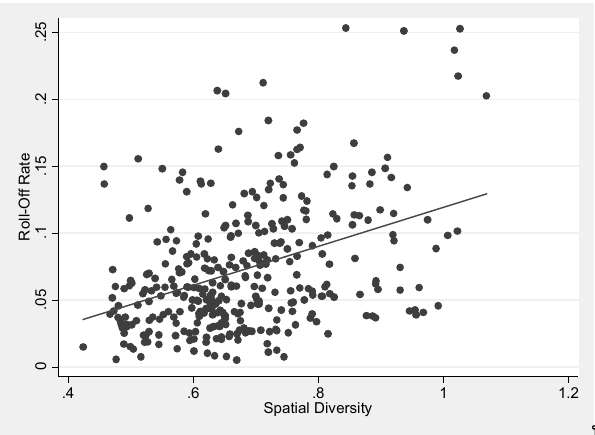
\includegraphics{img/sd_rolloff.png}
\caption{Effect of spatial diversity on electoral rolloff}
\end{figure}

\begin{figure}
\centering
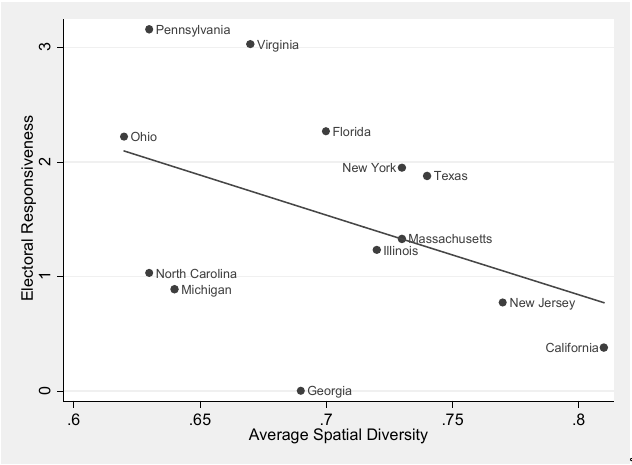
\includegraphics{./img/average_spatial-diversity.png}
\caption{Effect of electoral responsiveness on spatial diversity
\label{sd_responsiveness}}
\end{figure}

\begin{quote}
spatial diversity remained a statistically significant predictor of
roll-off rate. With these variables held constant at their means, a
House district's shift from the tenth to the ninetieth percentile in
spatial diversity was associated with an increase in roll-off rate of
about six percentage points.
\end{quote}

Electoral responsiveness refers to the rate at which a party gains or
loses seats given changes in its statewide vote share. For instance, if
Democrats would win ten percent more seats if they received five percent
more of the vote, then a plan would have a responsiveness of 2.0. As a
general matter, the lower a plan's bias, and the higher its
responsiveness, the better the plan is thought to be.

The story with responsiveness is more straightforward. As the se- cond
chart illustrates, responsiveness simply tends to decrease as aver- age
spatial diversity increases. The states whose districts are most
homogeneous, on average, are also the states whose elections are most
responsive to changes in public opinion. In contrast, the states whose
districts are most heterogeneous are also the ones in which even large
swings in voter sentiment have little impact on the parties' seat
shares. This finding indicates that while high spatial diversity is not
a prereq- uisite for a partisan gerrymander (low spatial diversity can
also do the trick), it is indeed an effective way to protect incumbents
of both parties from shifting political tides. \textbf{Advocates of
responsive elections, then, may push without hesitation for spatially
homogeneous districts to be drawn, since it is these districts that seem
most likely (in the aggregate) to reflect the public's evolving
preferences.}

\cite{steph2012}

\hypertarget{how-compactness-might-affect-spatial-diversity}{%
\subsubsection{How compactness might affect spatial
diversity}\label{how-compactness-might-affect-spatial-diversity}}

\hypertarget{previous-work}{%
\subsubsection{Previous work}\label{previous-work}}

\begin{itemize}
\tightlist
\item
  people have done how compactness affects competitiveness (schutzman
  2020)
\item
  people have used MCMC approach to look at how districts are more or
  less competitive ( daryl's work)
\end{itemize}

One factor ignored in this analysis, which is critical to theprocess of
drawing districts, isrespecting communities-of-interest.Even defining
and locating geographically such communities is avery difficult problem,
let alone the determination of whether ornot to preserve that group in a
single district. We therefore pro-pose our analysis as a framework for
discussion about trade-offs inredistricting rather than as a policy
recommendation.

In this work, we have demonstrated with a simple model thatdemanding
districts be drawn to be as compact as possible anddemanding that they
satisfy a notion of partisan symmetry areincompatible, but to different
degrees depending on the particularfeatures of the geographic region in
question. Since existing propos-als and methodologies for automated and
algorithmic redistrictinginvolve finding an approximate solution to an
optimization problem,it is important to understand how changing the
objective functionof these procedures can affect the outcome. As more
jurisdictionsconsider redistricting reforms, they should be cautious
about abdi-cating the line drawing process to algorithms which encode
valuesdifferent from those of the voters who use the districts to elect
theirrepresentatives.

\hypertarget{key-research-questions}{%
\subsection{Key research questions}\label{key-research-questions}}

\begin{enumerate}
\def\labelenumi{\arabic{enumi}.}
\tightlist
\item
  Is there an inherent trade-off between compactness and homogeneity?

  \begin{itemize}
  \tightlist
  \item
    Do more compact districts have better, equal, or worse spatial
    diversity scores?
  \item
    Does it depend on the compactness metric we use?
  \end{itemize}
\item
  Does spatial diversity give us a normative basis to select one
  compactness metric over another?
\end{enumerate}

\hypertarget{research-procedure}{%
\subsection{Research procedure}\label{research-procedure}}

To answer my research questions, I adopt the following procedure:

\begin{enumerate}
\def\labelenumi{\arabic{enumi}.}
\tightlist
\item
  Generate a large and representative subset of plausible districting
  plans
\item
  Evaluate compactness and spatial diversity scores on that subset of
  plans
\item
  Analyse the overall relationship between compactness and spatial
  diversity
\end{enumerate}

This three-step procedure is used by many previous works, including
\cite{cr2013}, \cite{ddj2019comp}, and \cite{s2020}. While the specifics
differ, they all follow the same general procedure. I will now explain
why this procedure has its advantages over more traditional political
science methods.

\hypertarget{why-generate-many-plausible-districting-plans}{%
\subsubsection{Why generate many plausible districting
plans?}\label{why-generate-many-plausible-districting-plans}}

I use a Markov Chain Monte Carlo (MCMC) approach to generate tens of
thousands of counterfactual districting plans. One might ask: What is
the point of using a simulation approach? Why not just use historical
districting plans that actually existed in real life? There are two
reasons. Firstly, there have not been very many historical districting
plans. There may be at most twenty districting plans over the history of
a state, but they range from the 1800s to the 2000s, and it would be
difficult---if not impossible---to get accurate data on these historical
plans. But the biggest problem in trying to draw a link between
districting plans and any outcome of interest is that of endogeneity.
Suppose we believe that plans with greater compactness lead to greater
political participation:

\[Compactness \rightarrow Participation\]

To answer this question, we could look at a couple of enacted
districting plans and measure their compactness and political
participation. Then we would be able to run an OLS regression and
retrieve the coefficients. But these coefficients would not have a
causal interpretation. We know that compactness is a result of
districting procedures that are political in nature. Political
participation affects who wins the state, and the winning party then has
outsize influence on the next districting plan. The districting plans
affect the outcome of the election, which in turn affects future
districting plans. This makes it incredibly difficult to find the
marginal effect of an increase in compactness on participation.

Even finding natural experiments may not be enough to remove the
endogeneity. The Supreme Court has often struck down proposed
districting plans and forced parties to propose a new one. We can think
of this as an exogenous shock and calculate compactness and political
participation in both plans. But even this has knock-on effects. When
the Supreme Court strikes down a plan, it's safe to say that there will
be significantly increased media coverage on the proceedings---which
will surely affect interest and participation in the subsequent
elections.

It would be incredibly useful to vary compactness unilaterally while
knowing that that variation was not due to a previous change in
political participation. But this is precisely what simulation
approaches allow us to do. If the simulations are able to generate a
representative sample of all districting plans (a big caveat---more on
this later), then we can solve the problem of sample size and
endogeneity in one fell swoop.

A simulation approach is therefore advantageous due to the limitations
of our data. But the simulation procedure introduces several new
considerations. We need to choose two things in the procedure: a method
to generate districting plans, and a compactness metric to score these
districting plans. This choice is not arbitrary: different generating
functions and the choice of compactness metric can give very different
results. I now explain how I chose both of these.

\hypertarget{overview-of-compactness-measures}{%
\subsubsection{Overview of compactness
measures}\label{overview-of-compactness-measures}}

To empirically evaluate a trade-off between compactness and homogeneity,
we must first figure out how to measure compactness. I give a brief
overview of the different types of measures and explain the pros and
cons of each. I present a compactness measure that I develop and finally
explain my decision to use an ensemble of four compactness measures to
increase the robustness of my results.\footnote{I use the phrases
  ``compactness metric'' and ``compactness measure'' interchangeably.}

Over a hundred compactness measures have been proposed in the
literature. Here, I focus on two main families: \emph{geometric}
compactness metrics and \emph{point-wise distance} metrics.

\hypertarget{geometric-compactness-metrics}{%
\paragraph{Geometric compactness
metrics}\label{geometric-compactness-metrics}}

Geometric compactness metrics are by far the largest class of
compactness measures. They look at some geometric properties of proposed
districts. These properties are most often shapes, area or
perimeter---although more esoteric measures do exist. Here, I explain
the three most popular compactness measures, although other popular
compactness measures e.g.~Schwartzberg are qualitatively similar.

\hypertarget{polsby-popper}{%
\subparagraph{Polsby-Popper}\label{polsby-popper}}

The Polsby-Popper measure is by far the most popular measure used in the
literature. It is the ratio of the area of the district to the area of a
circle whose circumference is equal to the perimeter of the district
\citep{pp1991}. A perfect circle has a Polsby-Popper score of 1.

\[4\pi \times \frac{A}{P^2}\]

\begin{figure}
\centering
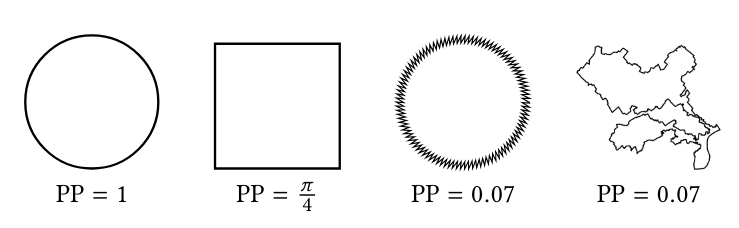
\includegraphics{img/pp_example.png}
\caption{Polsby-Popper scores of four example regions: a perfect circle,
a square, a circle with a ragged boundary, an an example district from a
Pennsylvania plan. Taken from \cite{s2020}.}
\end{figure}

\hypertarget{reock}{%
\subparagraph{Reock}\label{reock}}

The Reock score is a measure of the ratio of the district to the area of
the minimum bounding circle that encloses the district's geometry
\citep{reock1961}.

\[\frac{Area}{AreaOfMinimumBoundingCircle}\]

\begin{figure}
\centering
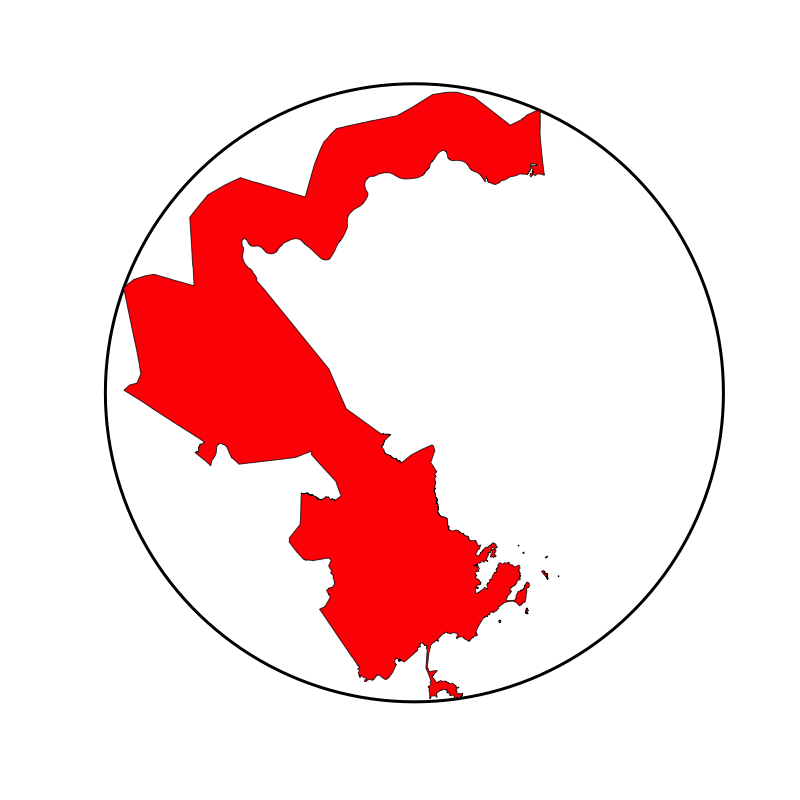
\includegraphics{img/reock.png}
\caption{A visualisation of the Reock metric.}
\end{figure}

\hypertarget{convex-hull}{%
\subparagraph{Convex Hull}\label{convex-hull}}

The Convex Hull metric is a ratio of the area of the district to the
area of the minimum convex polygon that can enclose the district's
geometry. A circle, square, or any other convex polygon has the maximum
Convex Hull score of 1.

\[\frac{Area}{AreaOfMinimumConvexPolygon}\]

\begin{figure}
\centering
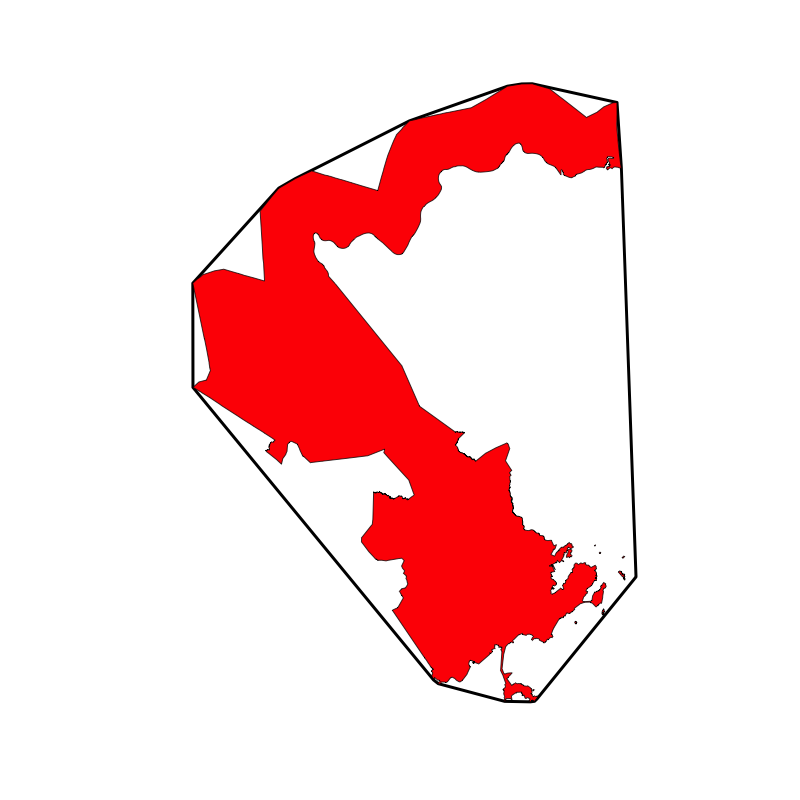
\includegraphics{img/ch.png}
\caption{A visualisation of the Convex Hull metric.}
\end{figure}

\hypertarget{choosing-a-compactness-metric}{%
\paragraph{Choosing a compactness
metric}\label{choosing-a-compactness-metric}}

Which compactness measure should we choose? All three compactness
measures are well-cited in the literature and enjoy widespread use. They
have been cited in U.S. Supreme Court cases, \emph{amici} briefs, and
redistricting commissions \citep{moncrief2011}.

Despite their widespread acceptance, however, the problems with
compactness measures are many, and well-covered in the literature. As an
example, the most popular compactness measure in the
literature---Polsby-Popper---is sensitive to small perturbations in data
resolution (the coastline problem).\footnote{The Polsby-Popper metric
  measures the ratio of the area of the district to the area of a circle
  whose circumference is equal to the perimeter of the district. But
  depending on the resolution of the map, the perimeter can be
  effectively infinite. \citeauthor{bswp} find that the choice of
  resolution has ``a substantial impact on compactness scores, with the
  Polsby-Popper score especially affected.''} The same is true for other
geometric compactness measures: no single metric is perfect. It is
therefore important to use an \emph{ensemble} of compactness measures to
make sure that one's data and conclusions are robust.

But even this is not enough. Because all three of these compactness
measures are purely geometric, they are all vulnerable to a specific
family of geographic perturbations. Indeed, \cite{bswp} show that
minimally tweaking the geometric features of states is enough for the
four most popular compactness measures (Polsby-Popper, Convex Hull,
Reock, Schwartzberg) to give very different conclusions on nominally
identical data.

Thus, it is important to include a non-geometric compactness measure in
the ensemble to guard against the possibility that the results are
driven by a specific quirk in geography. Many such measures have been
proposed. For instance, \cite{dc2016} bring in a discipline of
mathematics---graph theory---to formulate a new metric of compactness.
And \cite{kingwp} use a machine learning model to try and ape human
intuition---quantifying the intuitive metric of ``I know it when I see
it''.

\hypertarget{point-wise-distance-compactness-measures}{%
\paragraph{Point-wise distance compactness
measures}\label{point-wise-distance-compactness-measures}}

However, one particular class of metrics I term \emph{point-wise
distance} compactness stands out for its ease of understanding (critical
if it is to be persuasive to Supreme Court judges), theoretical
attractiveness, and academic consensus. Roughly speaking, this class of
compactness metrics tries to measure the distance between voters in a
district, and assigns higher scores the lower that distance is.

This class of metrics enjoys strong theoretical grounding. Paramount to
the idea of single-member districts is that there is some value in
voters who live in the same area being put into the same district.
\cite{er2019}:

\begin{quote}
``Voters in the same area are likely to share political interests;
voters in the same area are better able to communicate and coordinate
with one another; politicians can better maintain connections with
voters in the same area; voters in the same area are especially likely
to belong to the same social communities --- all suggest the importance
of voters being located in districts with their geographic peers.''
\end{quote}

In contrast, districts that put people with unrelated, faraway others
carve voters out of their natural communities and are thus to be
avoided. We care about whether co-districtors live in the same area and
belong to the same communities of interest, not just the compactness of
their electoral district. And point-wise distance metrics deliver
exactly that.

Therefore, point-wise distance metrics are more intuitive to laymen and
possess a normative bent that more abstract mathematical compactness
measures lack. It has therefore been an active area of development in
the literature. \cite{cm2010} present a measure of ``bizarreness'',
which is the ``expected relative difficulty in traveling between two
points within the district''. And \cite{fh2011} measures ``the distance
between voters within the same district relative to the minimum distance
achievable''.

Despite the relative merits of point-wise distance metrics, there are
two areas of improvement---one theoretical, the other empirical.
Firstly, all point-wise distance metrics suggested in the literature use
Euclidean distances. But many have rightly suggested that we should
consider travel times/driving durations instead. For instance, while
\cite{fh2011} used Euclidean distance in their metric, they point out
its shortcomings:

\begin{quote}
Suppose there is a city on a hill. On the West side is {[}a{]} mild,
long incline toward the rest of the city, which is in a plane. On the
East side is a steep cliff, either impassable or with just a narrow,
winding road that very few people use. While the next residential center
to the East is much closer to the hilltop on a horizontal plane, it is
much further on all sorts of distances that we think might matter:
transportation time, intensity of social interactions, sets of shared
local public goods and common interests, etc. Thus, for all practical
purposes, one probably wants to include the hilltop in a Western
district rather than an Eastern one. More general notions of distance
can handle this.
\end{quote}

The ``impassable'' region on the East would have a short Euclidean
distance, and any districting plan that put the hilltop with the Eastern
district would be unfairly penalised by these point-wise distance
metrics. On the other hand, the impassable region would have a long
driving duration, accurately reflecting the political geography. In this
and many other cases like it (e.g.~large bodies of water), driving
durations better reflect a state's unique political geographies.

After acknowledging the shortcomings of Euclidean distance,
\citeauthor{fh2011} specifically suggest using driving durations to
improve their metric: ``one can extend much of {[}our analysis{]} by
using driving distance or what legal scholars refer to as `communities
of interest'\,''.

There are thus strong theoretical grounds for using driving durations in
point-wise distance metrics. Why then have scholars not adopted it,
seeing as they agree on its superiority? This brings me to my empirical
criticism: the point-wise distance metrics scholars have proposed are
either far too computationally complex to compute at scale, or have
restrictions that make using travel times difficult, if not impossible.
For instance, the metric that \citet{fh2011} propose requires solving an
\emph{NP-complete} problem. A term used in computer science, an
NP-complete problem scales exponentially with the size of the input.
This makes it prohibitively expensive on larger states. And while they
have an approximation that runs much quicker, they provide no bounds on
the correctness of this approximation.

Similarly, \citeauthor{olson2010} has a metric that minimises the
average distance from each voter to the center of their district. He
says of travel times ``that it might be the right kind of thing to
measure, but it would take too long\ldots{} The large amount of map data
and extra computer time to calculate all those travel times would slow
the process down horribly. It would then require a room filling
supercomputer to get an answer in a reasonable amount of time.''
\citep{olson2010}. And finally, \citeauthor{cm2010}'s measure cannot
feasibly be improved with driving durations due to the difficulty of
finding point-to-point travel distances without passing through another
district. This is because most routing engines allow you only to specify
a route between two (or more) points. They do not further allow you to
specify regions through which the route cannot pass.

\hypertarget{an-improved-point-wise-distance-metric-human-compactness}{%
\paragraph{An improved point-wise distance metric: Human
compactness}\label{an-improved-point-wise-distance-metric-human-compactness}}

Given the difficulties of adapting existing point-based distance metrics
to use driving durations, I develop a new measure called \emph{human
compactness}. This metric incorporates driving durations at the very
outset, and builds in optimisations to run quickly. The human
compactness metric measures the ratio of driving durations between one's
nearest neighbours and one's fellow districtors. This ratio ranges from
0 to 1. The higher this ratio is, the more compact the district.
Intuitively, it encourages drawing districts that put one's next-door
neighbours together in the same district.

The human compactness metric works at three-levels: at the voter-level,
the district-level, and the overall plan-level. At the voter level,
human compactness of a voter is the ratio of: the sum of driving
durations to one's K nearest neighbours, to the sum of driving durations
to one's co-districtors, where K is the number of voters in that voter's
district. A simple example will be illuminating. The following figures
give a simple demonstration of how the human compactness metric is
calculated both on the voter- and district- level.

\begin{figure}
\centering
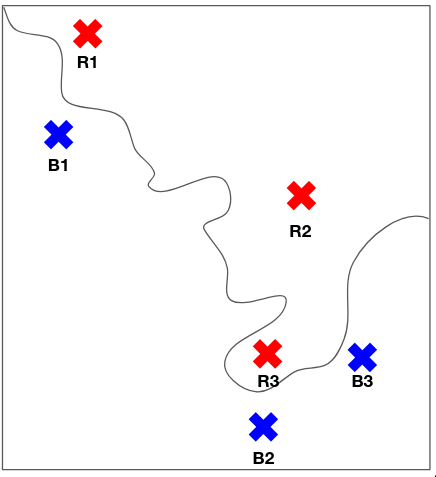
\includegraphics{img/human_compactness_1.png}
\caption{A simplified state assignment with two districts and six voters
\label{hc_demo}}
\end{figure}

Figure \ref{hc_demo} shows a highly simplified state assignment, with
two districts, Red and Blue, and three voters in each district. We label
each point from top-left to bottom-right. Note here that Red and Blue
are not partisan affliations: R1, R2 and R3 are red voters simply
because they happen to fall in the Red district.

We will first calculate the individual human compactness score for each
voter in the Red district. Figure \ref{hc_r1} illustrates this for the
top-left voter, R1. First, we find the sum of driving durations between
R1 and his fellow co-districtors R2 and R3. This sum, \(5 + 6\), forms
the denominator of the human compactness score.

\begin{figure}
\centering
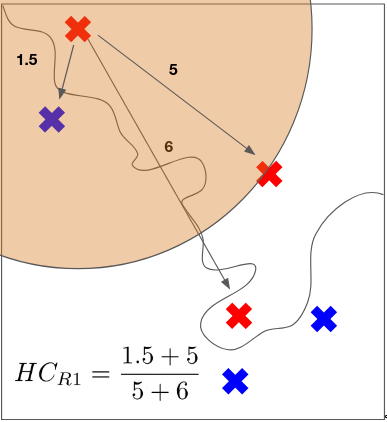
\includegraphics{img/human_compactness_2a.png}
\caption{Human compactness measure for voter R1 \label{hc_r1}}
\end{figure}

Next, we find the sum of driving durations between R1 and his nearest
neighbours. Because there are two other voters in his district, we will
find his two nearest neighbours. To find the two nearest neighbours,
here I have drawn a circle centered upon R1, and expanded the circle on
all sides until it touches two other voters. (This is not how the
algorithm works in reality)\footnote{The method of drawing an
  ever-expanding circle to get one's K-nearest neighbours only works for
  Euclidean distances. In reality, the ``circle of K-nearest
  neighbours'' will not be a circle, but rather be what is called an
  \emph{isochrone}: a line drawn on a map that connects points that have
  the same travel duration. The shape of the isochrone will vary with
  geographic features like cliffs or man-made features like highways. My
  implementation of the human compactness algorithm precomputes all the
  K-nearest neighbours for every single point, negating the need to
  calculate isochrones.}. We can see that R1's nearest neighbours are
the points B1 and R2, with a distance of 1.5 and 5 respectively. The
human compactness score of R1 is thus
\[HC_{R1} = \frac{d_{B1}+d_{R2}}{d_{R2} + d_{R3}} = \frac{1.5 +
5}{5+6} = 0.59\]

\begin{figure}
\centering
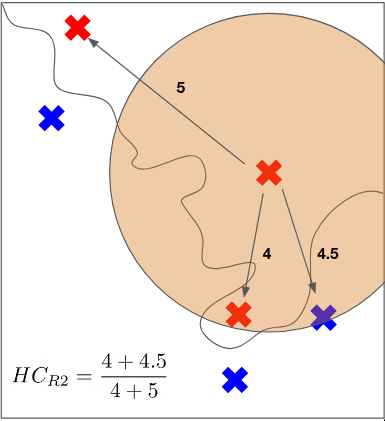
\includegraphics{img/human_compactness_2b.png}
\caption{Human compactness measure for voter R2 \label{hc_r2}}
\end{figure}

This is how we calculate an individual human compactness score. We
repeat the same procedure with R2 and R3, and obtain
\(HC_{R2} = \frac{4 + 4.5}{5+4}=0.94\) and
\(HC_{R3} = \frac{2 + 2.5}{4+6} = 0.45\). The compactness score for
point R3 is particularly low. We can see why this is the case in Figure
\ref{hc_r3}. Because point R3 is so close to B2 and B3, it really should
be put in the same district with them---R3 likely lives in the same
neighbourhood and/or community as B2 and B3. This is why the human
compactness metric gives it a very low score.

\begin{figure}
\centering
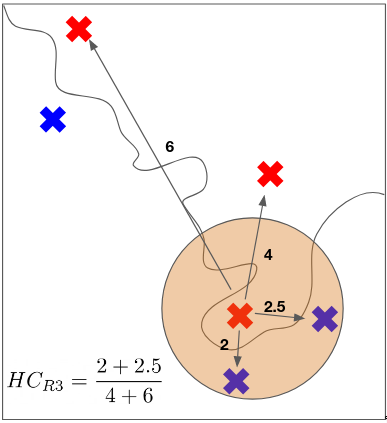
\includegraphics{img/human_compactness_2c.png}
\caption{Human compactness measure for voter R3 \label{hc_r3}}
\end{figure}

The \emph{district's} human compactness measure, \(HC_R\), simply takes
the ratio of all the sum of distances, as follows:\footnote{Another
  reasonable approach might be take the arithmetic mean of all
  individual human compactness scores. In that case the district-level
  human compactness score would be \(0.59 + 0.94 + 0.45 / 3 = 0.66\),
  basically identical to the value we obtained. I suspect that both
  approaches will give largely the same results.}

\[HC_R = \frac{(1.5+5) + (4 + 4.5) + (2.5 + 2)}{(5+6) + (5+4) + (4+6)} =
0.65\]

Finally, we obtain the districting plan's \emph{plan-level} compactness
score by taking the simple arithmetic mean of all district-level
compactness scores. Other aggregation functions are plausible: for
instance, taking the median, or the root-mean-squared value. In the
Results section, I run robustness checks with the root-mean-squared
aggregation function and find qualitatively similar results.

\begin{figure}
\centering
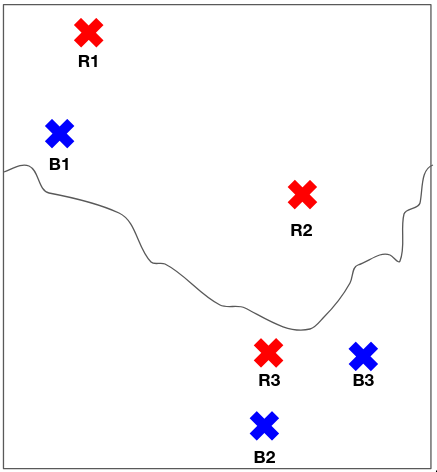
\includegraphics{img/human_compactness_3.png}
\caption{An alternative, more humanly compact proposed districting plan
\label{hc_better}}
\end{figure}

We have seen how to calculate the human compactness score for a proposed
districting plan. Now we demonstrate the conditions under which human
compactness score will assign better scores.

Figure \ref{hc_better} shows a proposed alternative districting plan.
Only the boundary has changed---the points have not. We can see
intuitively that this plan is more compact. Rather than being ``carved
out'' of his natural community in a snakelike fashion, R3 is now put in
a reasonably-shaped district with B2 and B3. We can calculate the
spatial diversity of this new district by imputing reasonable distance
values for R1--B1 and R2--B1. We thus get

\[HC_{R*} = \frac{(1.5 + 5) + (1.5+4.5) + (4 + 4.5)}{(1.5+5) + (1.5+4.5) + (5+4.5)} = 0.95\]

As we can see, the new district (and by extension districting plan) is
given a much higher score under the human compactness metric, which
largely accords with our intuitions. The human compactness measure
enjoys two significant advantages over existing approaches. First, the
human compactness metric improves upon the algorithmic complexity of
\citeauthor{fh2011}'s algorithm from an NP-hard problem to one with a
\(O(n^2)\) polynomial runtime. This is an exponential decrease in
algorithmic complexity. I also use programming techniques like
precomputation and memoisation to decrease the time taken to compute the
metric greatly. My implementation is competitive with geometry-based
compactness measures like Reock: on my machine, both metrics took
roughly the same amount of time (\textasciitilde{}0.20s per step). This
greatly increases the capability of political science researchers to
conduct ensemble analysis without requiring ``room-filling
supercomputers''. Further details on these algorithmic optimisations can
be found in Appendix A.

Because of these algorithmic improvements and the way I have designed
the metric, I am able to use driving durations rather than Euclidean
(as-the-crow-flies) distances between voters. This is a large
improvement with strong theoretical and empirical support. Many previous
scholars have suggested exactly this, giving it strong theoretical
support. It keeps the metric robust to quirks in political geography
like mountains and lakes, and better represents the notion of natural
communities. Empirically, too, the use of driving durations seems
strictly superior in many cases involving human-scale distances. Working
with Nicholas Eubank and Jonathan Rodden, I update their
gerrymandering-detection metric to use driving durations instead
\citep{er2019}. We find a consistently different picture of the social
context of American suburban voters, raising the possibility of false
positives under the Euclidean distance measure \citep*{elrwp}.

Given these considerations, I settle on an ensemble of four different
compactness measures: Polsby-Popper, Reock, Convex Hull, and Human
Compactness. I exclude the Schwartzberg metric as the Schwartzberg and
Polsby-Popper measure are largely mathematically equivalent. Finally, I
include the human compactness metric. This maximises the robustness and
validity of my results.

\hypertarget{generating-plans-with-automated-districting-algorithms}{%
\subsubsection{Generating plans with automated districting
algorithms}\label{generating-plans-with-automated-districting-algorithms}}

In order to find out whether compactness measures track spatial
diversity, we have to generate many counterfactual plausible plans that
span the entirety of possible districting plans and measure the
correlation between compactness and spatial diversity. This requires
using a computer to draw a large number of plans according to some
criteria.

The idea of drawing a large number of districting plans with a computer
has a long and storied history, starting in the 60s and 70s. The
approach has almost always been used to identify gerrymandering; for
instance \cite{ccd2000} build an algorithm to ``quantitatively
{[}assess{]} whether the {[}1990 South Carolina{]} plan is a racial
gerrymander''. More recently, \cite{cr2013} ``generat{[}e{]} a large
number of hypothetical alternative districting plans that are blind as
to party and race, relying only on criteria of geographic contiguity and
compactness.'' They do this using a Markov Chain simulation algorithm, a
procedure that makes iterative changes for a large number of steps until
a unique districting plan emerges. At each step of
\citeauthor{ccd2000}'s algorithm, they randomly select a Census Block
Group to serve as a ``seed'' of the district, then randomly add its
neighbouring block groups to it until a district with the desired
population is formed. Similarly, \citeauthor{cr2013} begin by
initialising all voting precincts as an individual, separate district,
then randomly agglomerating neighbouring precincts until the desired
number of districts is reached.

While this standard iterative algorithm enjoys a certain degree of
success, it has one crippling weakness. The way in which this class of
algorithms operates necessarily explores only a tiny subset of all
possible districting plans. Subsequent work pointed out this flaw:
\citeauthor{mm2018} wrote that automated processes ``may take a biased
sample of all possible legislative maps\ldots{} and fail to efficiently
produce a meaningful distribution of all alternative maps''. And
\citeauthor{fifieldwp} contend that ``{[}standard Monte Carlo
algorithms{]} are unlikely to yield a representative sample of
redistricting plans for a target population.'' \footnote{See
  \cite{fifieldwp}, pg. 16, for a technical explanation of why these
  algorithms don't produce uniform redistricting plans: ``For example
  \ldots{}, the creation of earlier districts may make it impossible to
  yield contiguous districts. These algorithms rely on rejection
  sampling to incorporate constraints, which is an inefficient strategy.
  More importantly, the algorithms come with no theoretical result and
  are not even designed to uniformly sample redistricting plans.''} This
poses a huge issue for the validity of any statistical analysis, because
any correlation that we discover on a biased subset of plans may be
spurious when measured over the actual distribution of plans. \footnote{Generating
  a biased sample is not necessarily a problem if all you want to do is
  \emph{optimise}, e.g.~draw the most compact plan possible. Recent work
  builds upon this standard algorithm, using Voronoi diagrams or
  iterative flood fill procedures rather than random chance, to assign
  the precincts to be agglomerated. See \cite{lf2019} for a technical
  overview.}

\hypertarget{markov-chain-algorithms}{%
\paragraph{Markov Chain algorithms}\label{markov-chain-algorithms}}

Thankfully, scholars have developed an improvement over the standard
algorithm with stronger theoretical guarantees. This second class of
algorithms reframe the districting problem as a \emph{graph partition}
problem (borrowing insights from graph theory and computer science), and
use a \emph{Markov Chain Monte Carlo} (MCMC) approach to sample possible
districting plans. This approach is best laid out in \cite{fifieldwp}.
The approach first initialises a specific graph partition. A graph
partition is an assignment of Census Tracts/Blocks to districts ---
basically a districting plan. This is the first step of the Markov
Chain. Then it \emph{flips} a random node of the graph to get another
valid partition. This process is repeated until the Markov Chain
approaches its steady state distribution: when this happens, the Markov
chain is called ``well-mixed''.

This class of algorithms inherit desirable well-known theoretical
guarantees of the Markov Chain.\footnote{See \cite{ddj2019recom} for a
  technical overview.} They are therefore much less likely (both
theoretically and empirically) to generate a biased subset of plans.
Conducting a small-scale validation study on a 25-precinct set,
\citeauthor{fifieldwp} compare the distribution of plans generated by
their algorithm to those generated by the standard redistricting
algorithm. They prove that their algorithm produces plans that hew much
more closely to the \emph{actual} distribution of all possible
districting plans.

Due to the many advantages of the MCMC approach, I use it in all my
analyses. However, there are many ways to conduct an MCMC analysis. The
key question is how one should sample from the near-infinite pool of
possible plans. State-of-the-art literature in this space use one of
three main approaches, all of which have their pros and cons.

The first is to get a sense for the properties of extremely compact
plans under each compactness measure by using a local optimization
technique, starting at a whole bunch of different initial seeds using
the single node \texttt{Flip} proposal. This approach gives us the most
compact plans, and is often used to find the ``maximal'' or ``best''
districting plans. However, it will---by design---only explore a very
tiny subset of all plausible districting plans. Also, because the
\texttt{Flip} proposal is very state-dependent, the initial state can
affect the results greatly.

The second is a middle-of-the-road approach, using a global proposal
distribution and a Metropolis-Hasting acceptance function to sample from
a distribution over plans that is proportional to
\(e^{(-\beta \times Compactness)}\). This will give us a distribution of
plans that is biased towards compact ones, but also contains some
noncompact plans.

One can get different distributions of plans depending on the specific
acceptance (score) function. For instance, \cite{dd2019va} prioritises
plans that have fewer locality splits and/or sustain a Black
majority-minority district. \cite{h2018} use a complicated score
function that takes into account county splitting, population deviation,
compactness and minority representation. If I were to use this approach,
I would define four different score functions corresponding to the
different compactness measures, and compare the resulting distributions
that result from each measure.

Finally, one can sample from a distribution that doesn't incorporate any
compactness score at all and extract the plans that achieve a good score
under each metric. This approach is used in \cite{ddj2019comp}, where
they generate a large neutral ensemble of districting plans and then
subsequently filter the plans according to increasingly strict vote-band
constraints. The advantage of this approach is that it casts the widest
net: all plausible districts (subject to the equal population bound) are
explored. The disadvantage is that the odds of sampling an `optimal'
district are incredibly low, which makes it suboptimal for algorithms
that aim to build the ``best'' plan.

\hypertarget{choosing-the-best-mcmc-approach}{%
\paragraph{Choosing the best MCMC
approach}\label{choosing-the-best-mcmc-approach}}

I use the third approach in my analysis.

The first proposal is local optimisation. Local optimisation approaches
like the \texttt{Flip} proposal have one key problem. The ``mixing
time'' of the Markov Chain under the \texttt{Flip} proposal---that is,
the number of steps it takes for the Markov Chain to be ``close enough''
to the stationary distribution---is very large. What that means is that
the \texttt{Flip} proposal tends to generate very uncompact, snakelike
districts in the beginning, as can be seen in Figure
\ref{recom_vs_flip}. It will take millions of steps for plans under the
\texttt{Flip} proposal to reach a satisfactory districting plan. As
such, I prefer the Recombination (Recom) distribution by
\citeauthor{ddj2019recom}, which uses a spanning tree method to
bipartition pairs of adjacent districts at each step
\citep{ddj2019comp}. This proposal distribution improves upon the
\texttt{Flip} proposal by decreasing the mixing time needed to reach a
satisfactory districting plan.

\begin{figure}
\centering
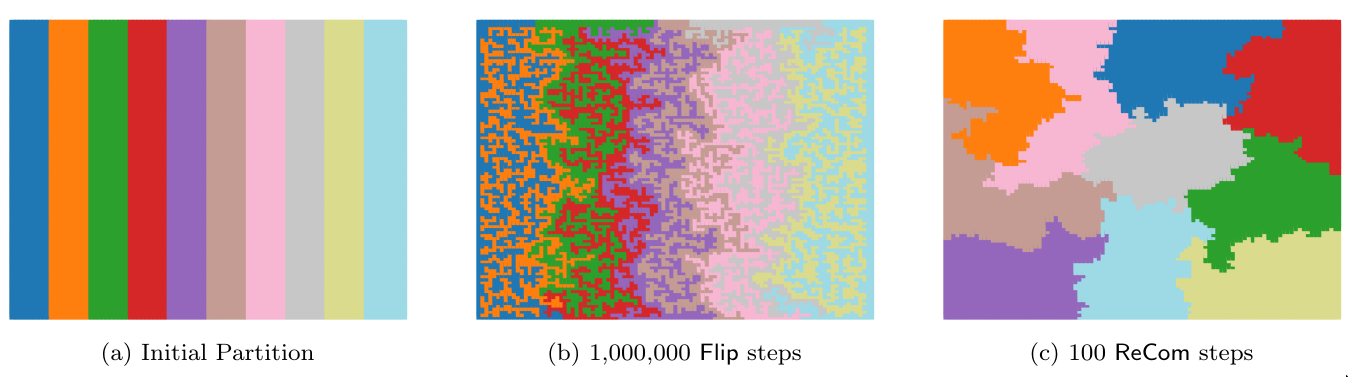
\includegraphics{img/recom_vs_flip.png}
\caption{\label{recom_vs_flip} The \texttt{Recom} proposal generates
more realistic plans in much fewer steps. Taken from
\cite{ddj2019recom}.}
\end{figure}

Mixing time aside, the extreme compactness of local optimisation is in
fact something that I want to avoid. I aim to find out if mandating
compactness in state constitutions can inadvertently adversely affect
democratic representation. But restricting one's analysis to extremely
compact plans deals a huge blow to the external validity of any such
finding. Redistrictors care about a lot of other considerations apart
from compactness, and therefore most definitely do not optimise solely
over compactness. State constitutions demand that plans be ``reasonably
compact'', not ``maximally compact'': it's vanishingly unlikely that
those extremely compact plans would resemble the types of plans that
would be drawn in real life. As such, \emph{even} if I found that
optimally compact plans had greater spatial diversity, this would have
very little bearing on redistricting policy. It's far more instructive
to see whether the relationship holds in the plans that legislators
could actually be expected to draw.

\begin{center}\rule{0.5\linewidth}{\linethickness}\end{center}

Given that legislators care a lot about many different considerations,
might it be better to try and include these considerations into the
score function? This is what the second approach does. While this
approach holds strong theoretical merit, I find that this approach
introduces too many degrees of freedom. The choice of what factors to
include in the score function is contentious: \citeauthor{h2018} use
population deviation, Polsby-Popper score, county boundaries and
minority deviation. But they could just as easily have included factors
such as proportionality or number of cut edges (proposed in
\cite{dc2016}) for instance. Even if there is a strong justification for
including exactly those factors, there is still significant researcher
freedom to operationalise the scores. For instance, \citeauthor{h2018}
and \citeauthor{dd2019va} both include a population deviation score, but
operationalise the metric differently. Furthermore, any score function
has to be assigned specific weights--- but this assignment is somewhat
arbitrary and open to argument. For instance, \citeauthor{h2018} ``chose
a VRA score function which awards lower scores to districting plans
which had one district close to 44.48\% African-Americans and a second
district close to 36.20\% African-Americans'', on the basis that the
2016 districting plan which was accepted by the Court had districts with
those proportions. But this is incredibly arbitrary. Obviously, just
because a particular district was accepted by the Court with those
proportions of African-Americans doesn't imply that those exact
proportions of African-Americans are optimal.

To be clear, these problems are not insurmountable. If there is a strong
theoretical basis for one particular operationalisation over another,
then the criticism of researcher fiat largely loses its bite.
Furthermore, the results obtained are robust to a variety of
perturbations. \cite{h2018} change the weights and threshold values as a
robustness check and find qualitatively similar results. Nonetheless,
different results can occur. And if two different operationalisations or
factor weights yield qualitatively different results, how would we
adjudicate between them? For these reasons, I choose not to use the
second approach.

\begin{center}\rule{0.5\linewidth}{\linethickness}\end{center}

The last approach is one that makes the fewest assumptions. It generates
a neutral ensemble and does not favour one plan over another (except for
some minimal compactness and population deviation requirements). This
approach gives us the largest space of plausible plans, which has a key
advantage: it allows the results to be applicable even for districting
algorithms that do not use an MCMC approach. This includes not only the
regular low-tech way of drawing districts, but also other automated
districting algorithms like \cite{mm2018} and \cite{lf2019}.

Therefore, I elect to use the last, ``neutral walk'' approach. I use a
global \texttt{Recom} proposal to generate the states, but accept every
proposal subject to minimal population deviation requirements. This
gives me a neutral ensemble of 10,000 plans for every state.

\hypertarget{research-procedure-continued}{%
\subsection{Research Procedure
(continued)}\label{research-procedure-continued}}

Now that we have chosen both the compactness metric and the simulation
procedure, we can refine the previous three-step procedure into
something more specific:

\begin{enumerate}
\def\labelenumi{\arabic{enumi}.}
\tightlist
\item
  Use the Recom proposal function to generate a neutral ensemble of
  10,000 districting plans for every state
\item
  Calculate spatial diversity and four compactness scores
  (Polsby-Popper, Reock, Convex Hull, and Human Compactness) for each
  districting plan
\item
  Perform data analysis (OLS regressions, difference-in-means test) and
  obtain results
\end{enumerate}

I now describe each step in detail.

\hypertarget{generating-100000-districting-plans-with-the-mcmc-algorithm}{%
\subsubsection{Generating 100,000 districting plans with the MCMC
algorithm}\label{generating-100000-districting-plans-with-the-mcmc-algorithm}}

I download Census Tract data from the \href{census.gov}{United States
Census Bureau} website. I use Census Tracts rather than Census Blocks
because Census Tracts are the smallest (highest-resolution) units that
have spatial diversity data.

I use the open-source software library GerryChain to generate the
ensembles. Replication code and data are included in the Supplementary
Information. I obtain the ReCom Markov chain procedure from one of the
co-authors (Daryl Deford) of the \cite{ddj2019recom} paper. I then fed
the Census Tract data into the GerryChain library. Using the Recom
Markov chain procedure, I generated 10,000 districting plans for 10
states (Connecticut, Georgia, Idaho, Louisiana, Maine, Maryland, New
Hampshire, Rhode Island, Utah, and Wisconsin) for a total of 100,000
plans.

\begin{figure}
\centering
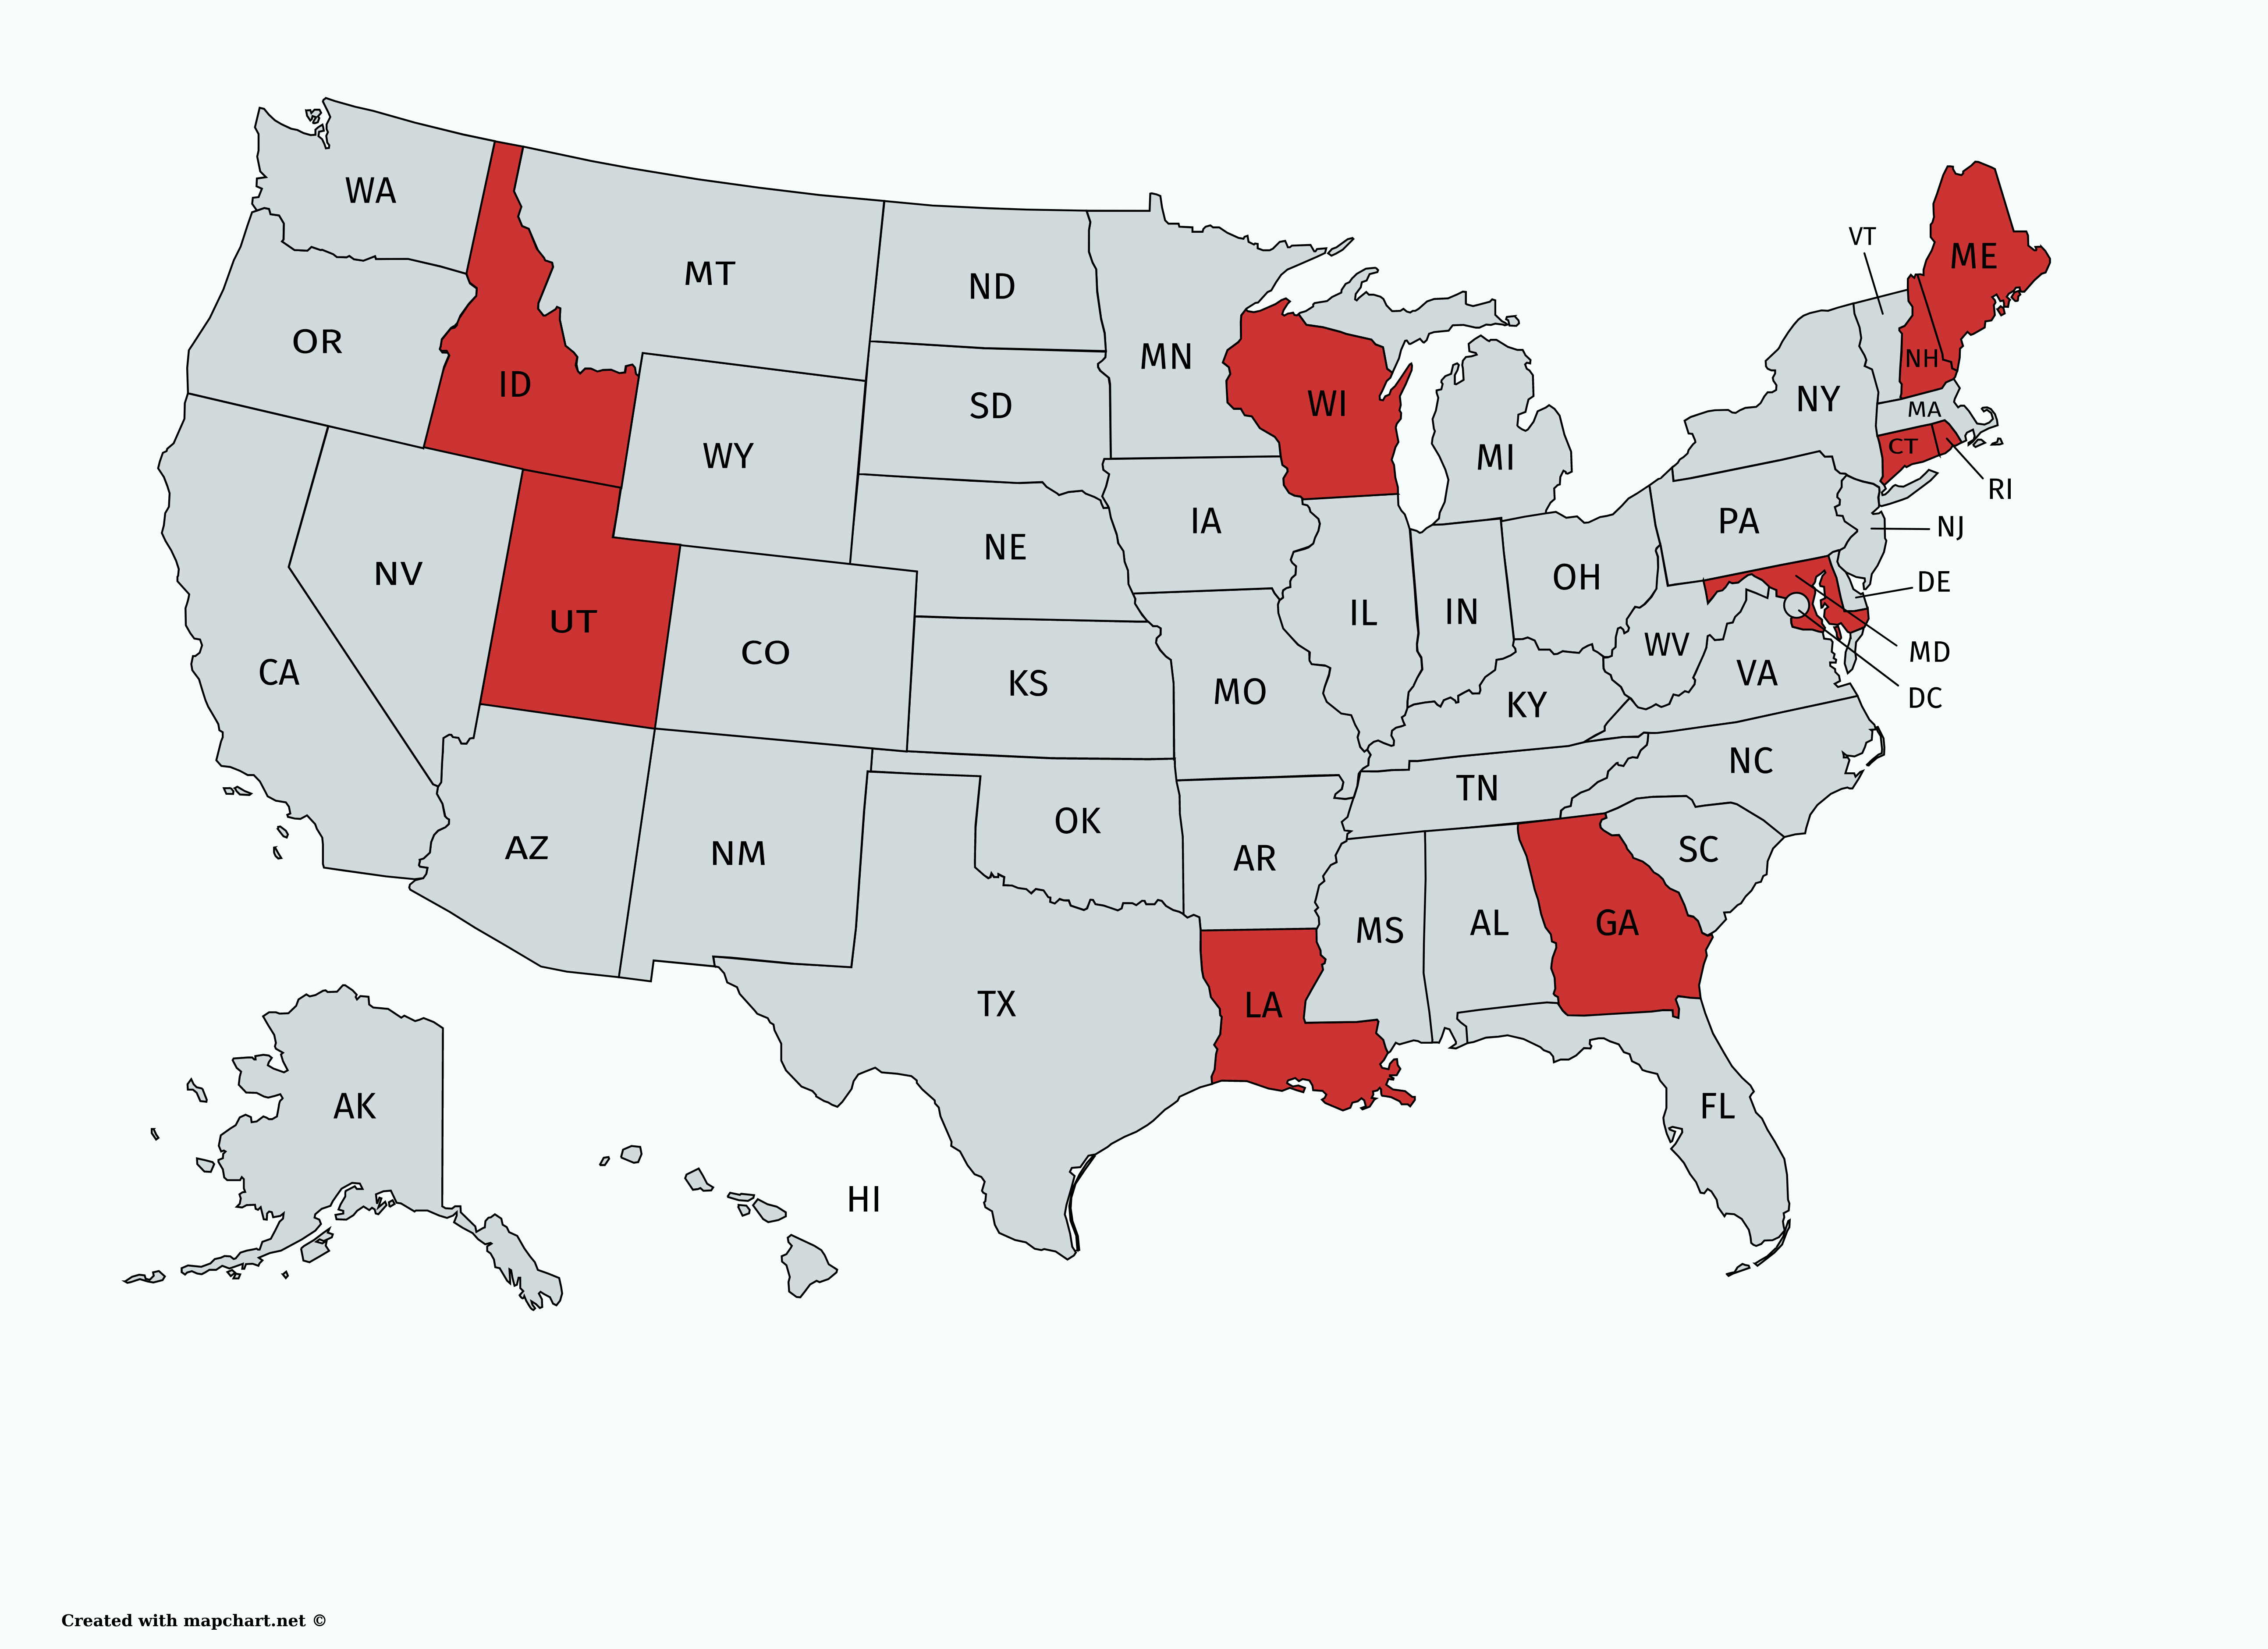
\includegraphics{./img/states_analysed.png}
\caption{States I analysed, marked in red \label{states_analysed}}
\end{figure}

Figure \ref{states_analysed} marks the states I analysed in red. I chose
these states mainly due to size considerations. All of these states are
small-to-medium sized (in terms of the number of Congressional
districts): the largest states like California, Texas and Florida are
absent. This is because my algorithm scales in both time and memory with
the \emph{square} of the size of the state (\(O(n^2)\)). The analysis is
achievable with larger desktop machines. Unfortunately, my own laptop
had only 8GB of RAM and not very much free disk space, making it
infeasible to examine larger states. Nonetheless, I was still able to
analyse medium-sized states like Louisiana, Maryland and Georgia (14
districts).

Size aside, I tried to get states that spanned the entire country,
including Western states (Idaho, Utah), Southern states (Louisiana,
Georgia), and Northeastern states (New England). I would also have liked
to generate plans from a Pacific state like Oregon and a Midwestern
state like Kansas, but time constraints prevented me from doing so.

Nonetheless, the number of states that I analyse exceeds most other
similar analyses. For instance, the seminal and heavily-cited work
\cite{cr2013} only analyse the state of Florida, and even very recent
work by \cite{ddj2019recom} and \cite{s2020} analyse only five and two
states respectively.

\hypertarget{calculating-spatial-diversity-and-compactness-scores-for-100000-plans}{%
\subsubsection{Calculating spatial diversity and compactness scores for
100,000
plans}\label{calculating-spatial-diversity-and-compactness-scores-for-100000-plans}}

After generating the plans, I calculate spatial diversity and
compactness scores for all of them. I obtain data on spatial diversity
from Professor Nicholas Stephanopoulos. The dataset he gave me has
\emph{factor scores} for each Census Tract in the country. A district's
spatial diversity score is calculated by the sum of the standard
deviation of each factor score, normalised by the proportion of the
variance each factor score explains. As an example, consider a district
made up of three Census Tracts (A, B, C), and let each Tract have three
factor scores (1, 2, 3). Let the proportion of the variance explained by
each factor score be 50\%, 30\% and 20\% respectively. Then the total
spatial diversity score would be:

\[ \sigma(A_1, B_1, C_1) \times 0.5 + \sigma(A_2, B_2, C_2) \times 0.3 + \sigma(A_3,
B_3, C_3) \times 0.2\]

I calculate spatial diversity score for every district, and, following
Stephanopoulos, take the arithmetic mean of all districts in a
districting plan to get the overall spatial diversity score for that
plan.

Next, I calculate compactness scores. As the Polsby-Popper metric is so
well-known and widely used, there was already an existing implementation
in the GerryChain library which I made use of. Similarly, existing
libraries like SciPy already had a Convex Hull method. Finally, I wrote
my own implementation of Reock, making use of the Smallest Enclosing
Circle code written by Project Nayuki \citep{nayuki2020}.

In order to calculate human compactness scores, I have to know where
voters live (to calculate driving durations between them). I therefore
obtain a dataset of ``voter representative points'' (VRPs) from
\cite{er2019}. These points aggregate many actual voters, downsampling
the data into a size that can be worked with. While this down-sampling
and placements of points randomly does introduce some noise, ``the
variability contributed\ldots{} is empirically very small''
\citep{er2019}. I sample 1,000 VRPs for each Congressional District in a
state. That means that a state like Maine with two districts will have
2,000 VRPs, and a state like Louisiana---with seven districts before the
new redistricting plan---will have 7,000.

I then calculate all pairwise driving durations between all VRPs using
an open-source routing engine called Open Source Routing Machine (OSRM)
built by \cite{osrm}. The routing engine is able to calculate driving
durations between any two points---very similar to Google Maps---but the
number of queries it can process is orders of magnitude larger than the
limits imposed by the Google Maps API. For these ten states, I calculate
about 400 million point-to-point driving durations in total. As point of
comparison, using Google Map's
\href{https://developers.google.com/maps/documentation/distance-matrix/usage-and-billing}{Distance
Matrix API} for that number of requests would cost \$1,480,000\footnote{Volume
  discounts do exist, but you have to contact the Sales Team, and I
  doubt I could afford it anyway\ldots{}}. And if I had tried to analyse
California (with 53 Congressional districts), this would require almost
3 billion point-to-point driving durations.

Because my analysis is on the tract level, I map VRPs to Census Tracts
using a spatial join. I sum the pairwise point-to-point distances to get
a matrix of pairwise \emph{tract-to-tract} driving durations. I then sum
the driving durations from each point in the district to another and
calculate the human compactness score for each district.

Finally, I aggregate the individual district scores into a plan-level
score by simply taking the arithmetic mean. For instance, if a
districting plan has three districts with Polsby-Popper scores of 0.25,
0.5, and 1, the Polsby-Popper score for that plan would be 0.5833. As a
robustness check, I also use the sum of square roots as an aggregation
function: that is,
\(\sqrt{0.25} + \sqrt{0.5} + \sqrt{1} = 0.736\)\footnote{This penalises
  districting plans that have a large difference between districts
  e.g.~one very good district and one very bad one.}, obtaining
qualitatively similar results.

\hypertarget{performing-data-analysis-on-the-100000-plans}{%
\subsubsection{Performing data analysis on the 100,000
plans}\label{performing-data-analysis-on-the-100000-plans}}

After calculating the overall spatial diversity and compactness scores
on all the plans, I start running exploratory data analysis and
statistical tests. The results are detailed below.

\hypertarget{results}{%
\subsection{Results}\label{results}}

My key results are as follows:

\begin{enumerate}
\def\labelenumi{\arabic{enumi}.}
\tightlist
\item
  Political geography largely pins down the spatial diversity of each
  individual district\footnote{Small urban districts have high SD, large
    rural ones have low SD.}.
\item
  Different compactness measures have different ideas of what ``good''
  plans look like.
\item
  Different compactness measures are correlated with one
  another\footnote{The geometric compactness measures agree most with
    one another, the human compactness measure not as much.}.
\item
  Only human compactness is negatively correlated with spatial
  diversity: geometric/dispersion-based measures have either no or a
  positive (bad) effect on spatial diversity\footnote{OLS regressions
    with state dummies show that only human compactness has a
    significantly negative coefficient on spatial diversity.
    Difference-in-means tests show that only the most compact plans
    under human compactness are less spatially diverse than average, and
    are less spatially diverse than the most compact plans under
    geometric/dispersion-based measures.}.
\end{enumerate}

Overall, the evidence suggests that optimising over compactness will
give you less spatially diverse districts, and human compactness will do
the best job of it.

\hypertarget{initial-analysis}{%
\subsubsection{Initial analysis}\label{initial-analysis}}

Before proceeding to more quantitative statistical tests, I want to show
what the generated plans look like and what the \emph{distribution} of
those plans looks like.

\hypertarget{the-best-and-worst-plans-according-to-different-compactness-measures}{%
\paragraph{The best and worst plans according to different compactness
measures}\label{the-best-and-worst-plans-according-to-different-compactness-measures}}

After having obtained all the plans and their corresponding scores, I
plot the plans with the best and worst spatial diversity and compactness
scores to get an understanding for the types of plans that each metric
encourages. This will give us valuable intuition for understanding the
subsequent results.

For ease of exposition I show states with only two districts, but the
analysis extends to states with any number of districts. (Plots of the
other eight states are available in the Supplementary Information). I
also use Polsby-Popper to represent the other two dispersion-based
compactness metrics as my explanations are similarly applicable to those
metrics.

\begin{figure}
\centering
\includegraphics{../30_results/33_min_max_subplots.png}
\caption{Best and worst districting plans of New Hampshire under
different metrics \label{nh_minmax}}
\end{figure}

\begin{figure}
\centering
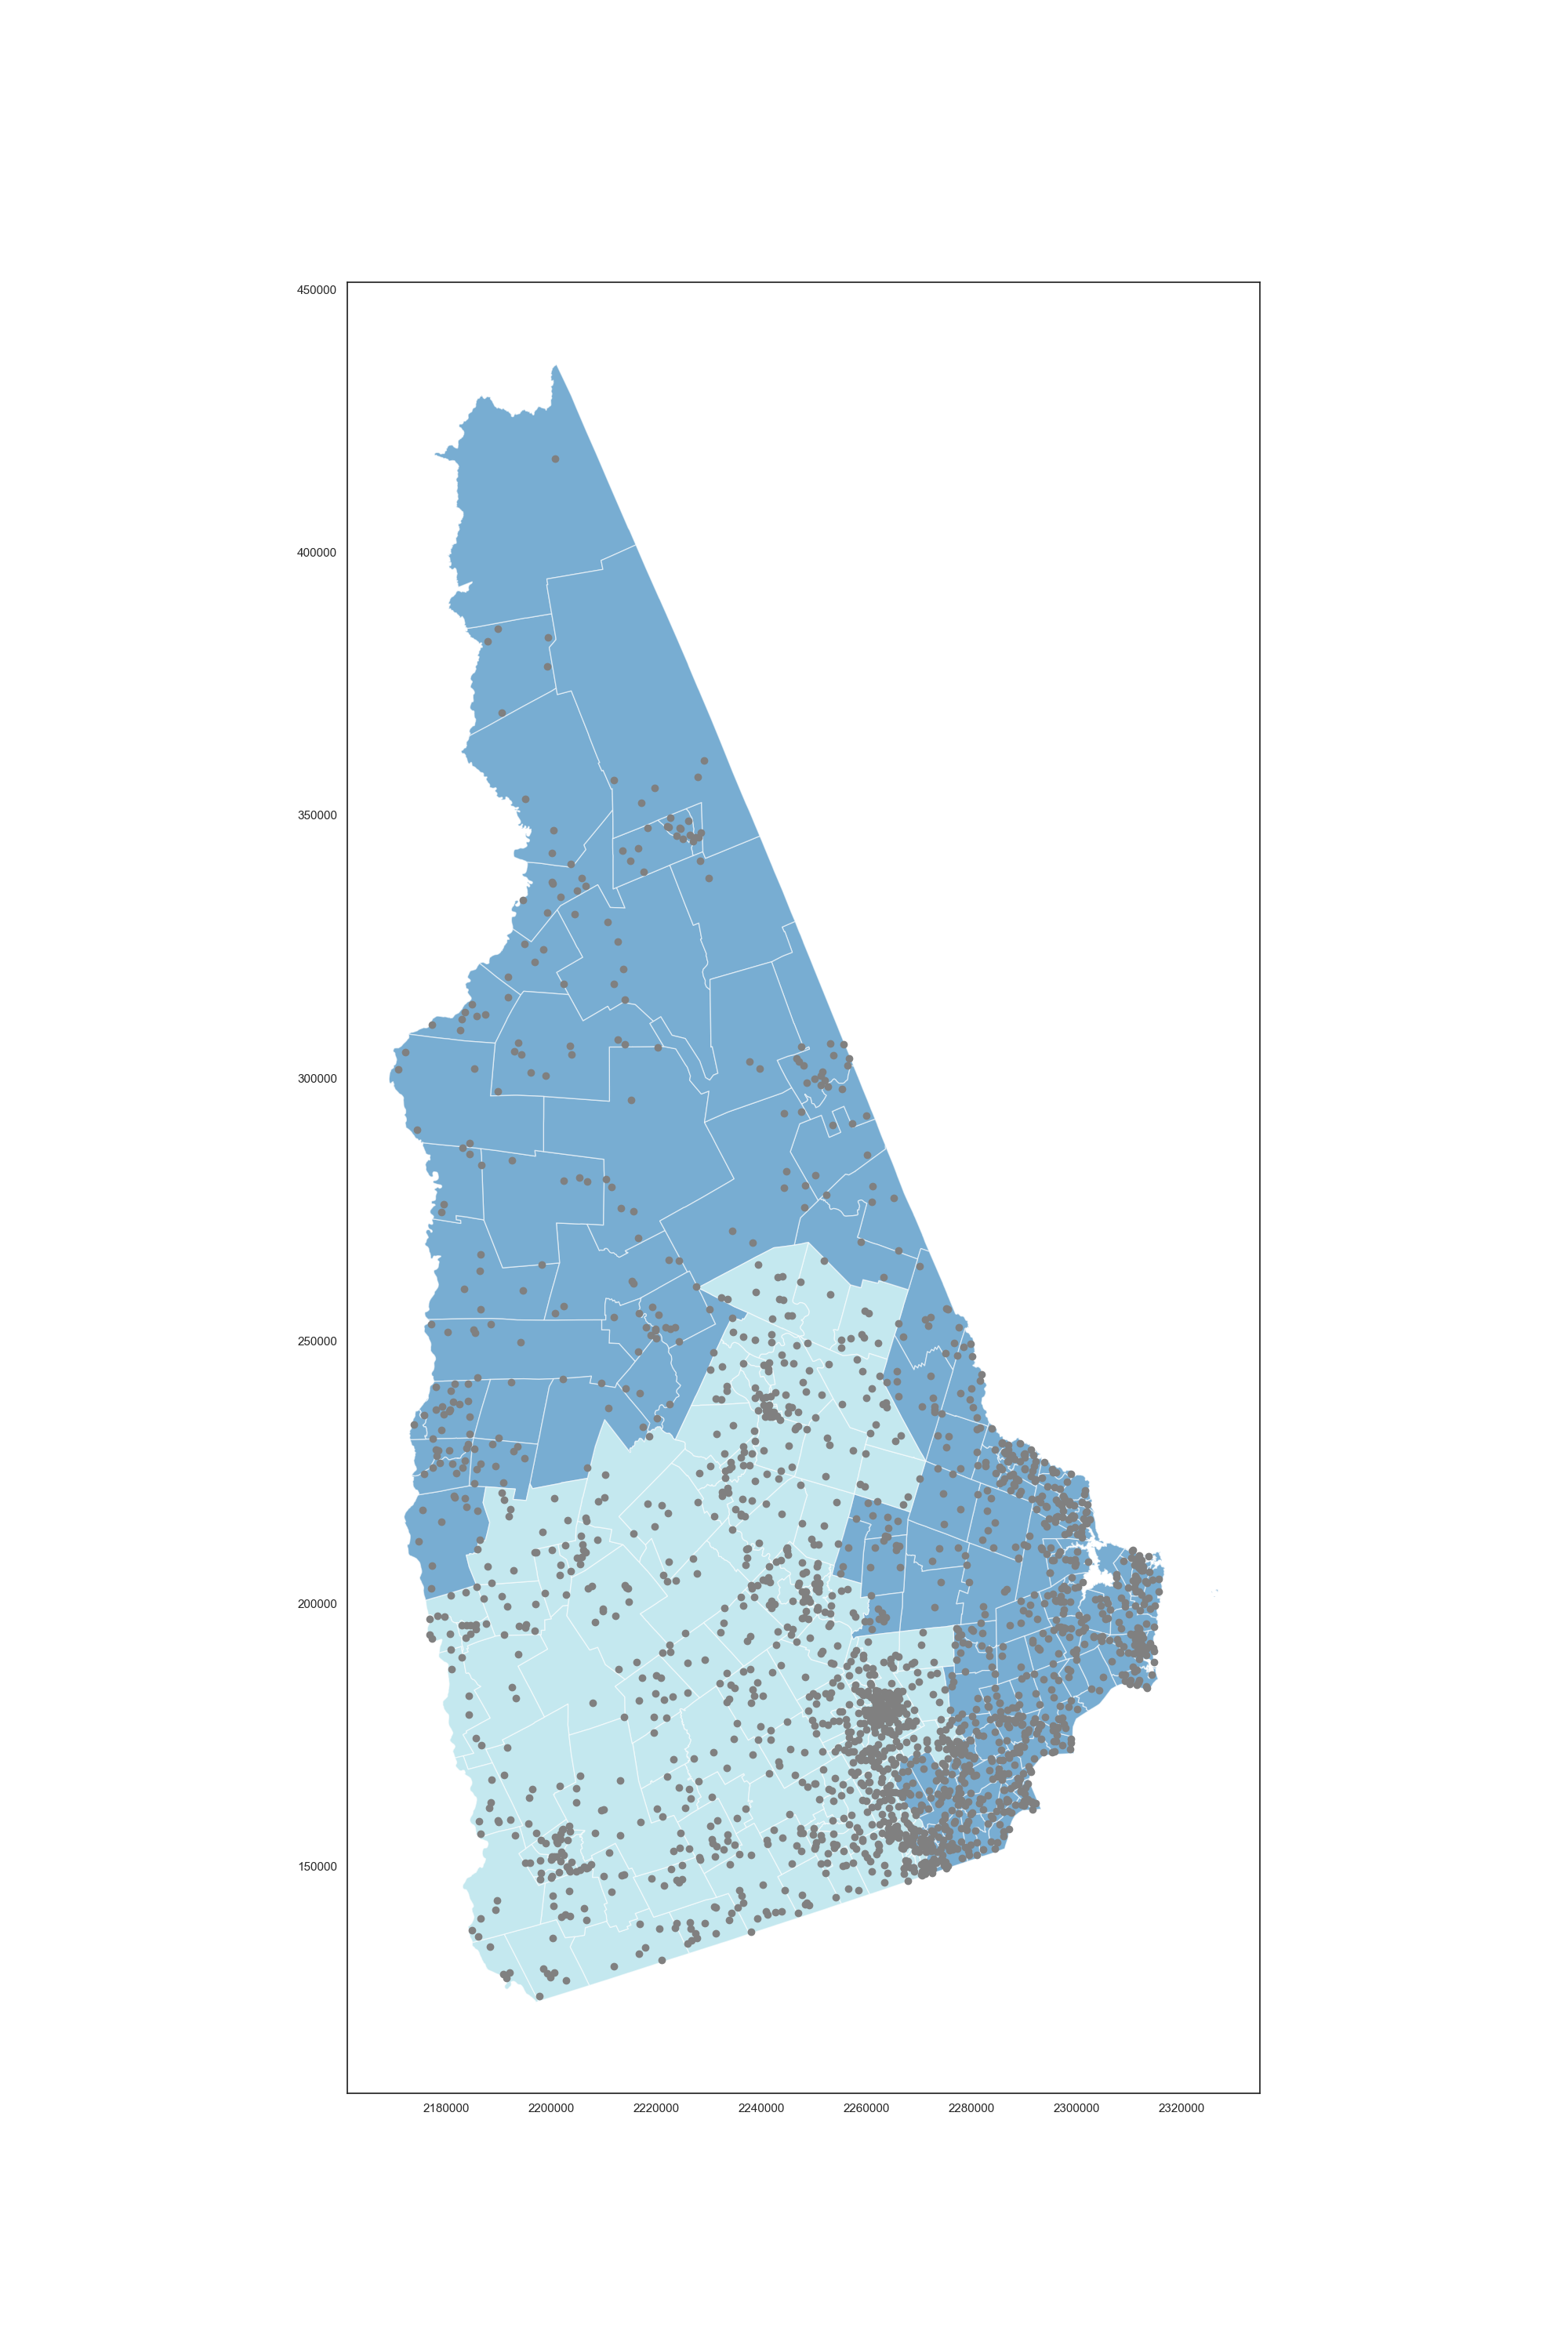
\includegraphics{../30_results/33_points_on_tracts.png}
\caption{Population density plot of New Hampshire. Each dot represents
roughly 600 people. \label{nh_density}}
\end{figure}

Figure \ref{nh_minmax} plots the best and worst plans according to
several metrics. Let us begin with the middle row (Polsby-Popper), as
its interpretation is the most straightforward. The Polsby-Popper (and
other dispersion-based) metric penalises districts that are very
``snakelike'' and prefers districts that have regular shapes like
squares or circles. This is clearly reflected in the plot. The best plan
has a district with a very regular shape, and the worst plan has a
snakelike district that contorts through half the state.

On the top row is human compactness. A good plan under human compactness
minimises the total travel times between every member of the district.
This encourages small, compact districts that avoid splitting urban
centers.

We can see that the top plan under human compactness corresponds well to
the actual population density of New Hampshire as seen in Figure
\ref{nh_density}. The top plan puts the two most populous and urban
counties in New Hampshire---Rockingham and Hillsborough---together in
the same district. The worst plan under human compactness splits the
counties in such a way that one's co-districtors are far away, and one's
nearest neighbours are in a separate district.

As expected, the top plan under spatial diversity (bottom row) closely
resembles the top plan under human compactness. In relatively
homogeneous New Hampshire, the main source of spatial diversity is the
urban-rural divide. A plan that keeps urbanites together in one district
is favoured under spatial diversity.

And while the worst plan under spatial diversity looks different from
that under human compactness at first glance, they are actually quite
similar. Both plans split up the two populous urban counties, having a
``fish-hook'' shaped district that starts from the rural north of the
state and swoops down to the south to carve out a large part of the
counties.

This case study shows that dispersion-based measures may not always
reflect existing communities of interest. This seems to fuel criticism
of dispersion-based measures on exactly that basis (``it makes no sense
to combine areas that have nothing in common except that they fit neatly
into a square'' \citep{wolf2015}). In this example, human compactness
and spatial diversity agree neatly on what the best districting plans
should look like.

While human compactness generally tracks spatial diversity better than
other compactness metrics (I provide evidence for this later), it does
not always do so. Figure \ref{idaho_density} gives the population of
Idaho. We can see that a large proportion of the population is
concentrated in a U-shaped ``belt'' spanning the southern half of the
state. A good plan under spatial diversity will attempt to put this
relatively urban ``belt'' in the same district, and this is indeed what
we observe in Figure \ref{idaho_minmax}. But due to its great distance
and jagged perimeter, such a plan is penalised under both human
compactness and dispersion-based measures, both of which prefer a
relatively compact square-shaped district.

\begin{figure}
\centering
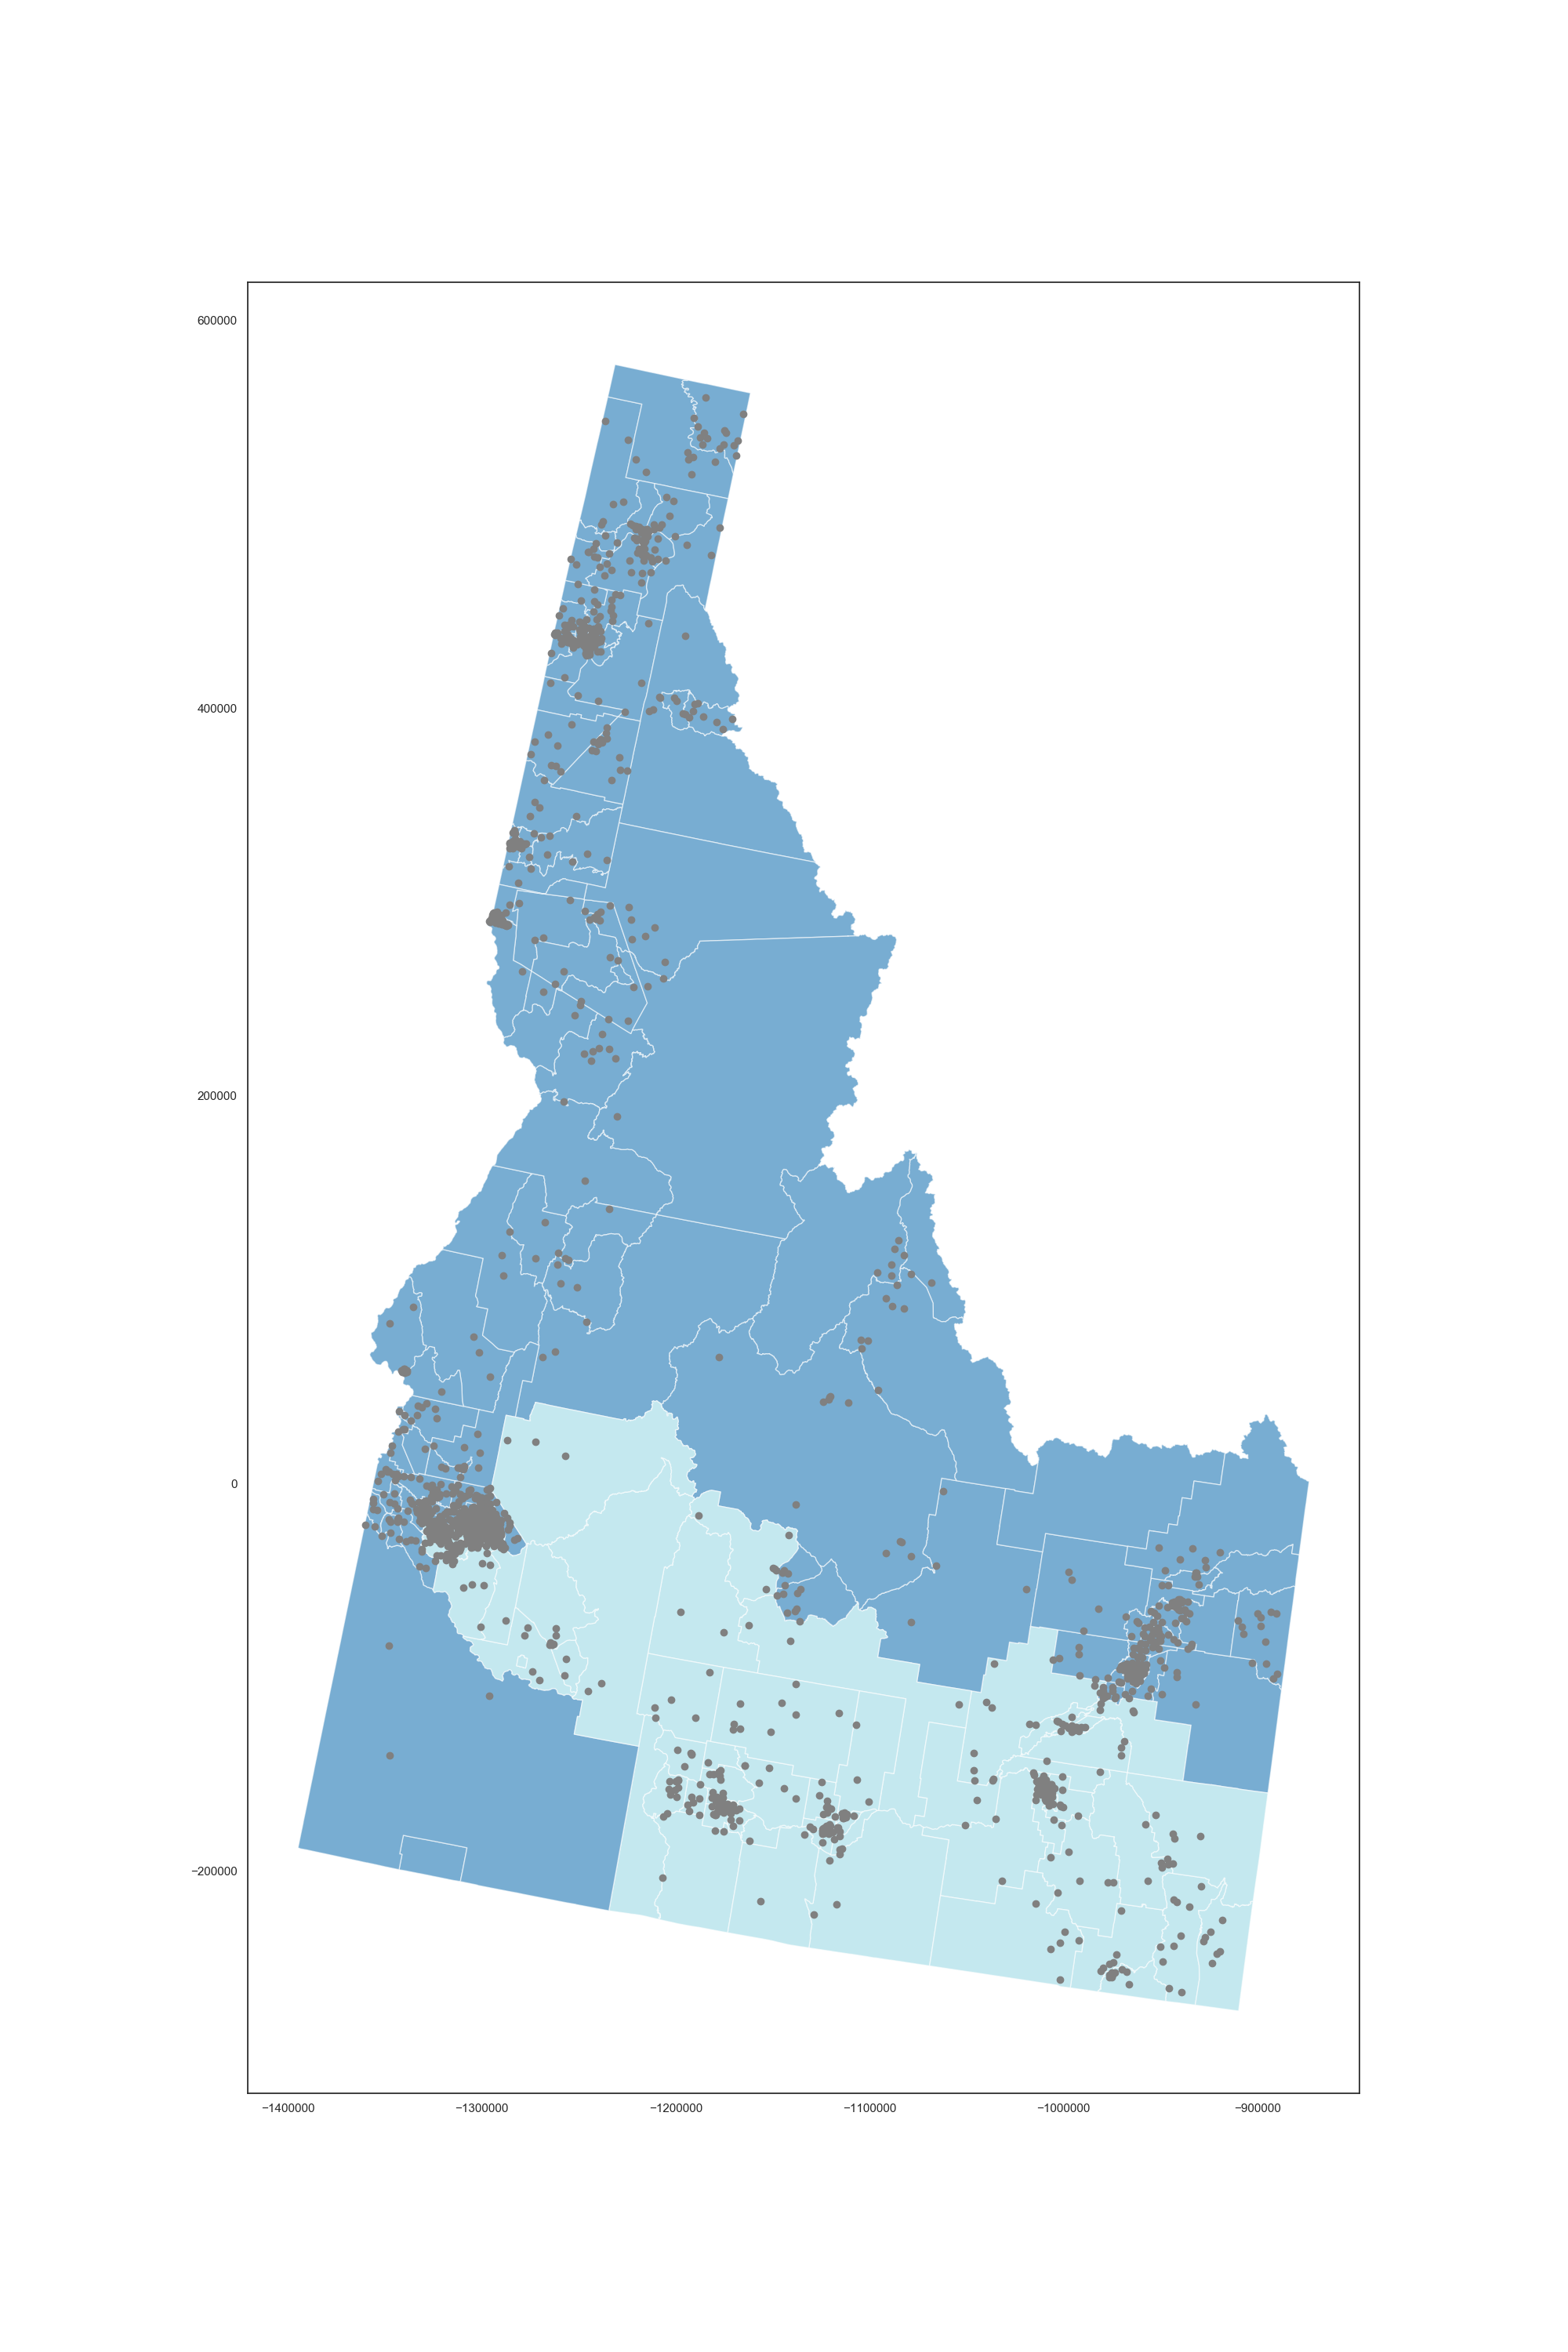
\includegraphics{../30_results/16_points_on_tracts.png}
\caption{Population density plot of Idaho. Each point represents
\textasciitilde{}700 people. \label{idaho_density}}
\end{figure}

\begin{figure}
\centering
\includegraphics{../30_results/16_min_max_subplots.png}
\caption{Best and worst districting plans of Idaho under different
metrics \label{idaho_minmax}}
\end{figure}

As we can see, compactness measures need not always agree with spatial
diversity, particularly in the case study of Idaho. Intuitively, this
seems to make sense: spatial diversity tries to put similar people
together, and people who live in the same area are often, but not
always, similar.

\hypertarget{political-geography-pins-down-the-spatial-diversity-of-each-individual-district}{%
\subsubsection{Political geography pins down the spatial diversity of
each individual
district}\label{political-geography-pins-down-the-spatial-diversity-of-each-individual-district}}

In this section, I show that spatial diversity varies enormously between
districts, but this is to a large extent dependent on the state's
political geography. I find that small urban districts have high spatial
diversity, while large rural ones have low spatial
diversity---regardless of districting plan. This also extends to the
level of the state: while the spatial diversity of districting plans can
range from 0.4 to 0.9, the spatial diversity of a state's districting
plan usually lies within a small range of \textasciitilde{}0.05.

Figure \ref{sd_all_districts} is a kernel density estimation (KDE) plot
of the distribution of spatial diversity in all districts. As in
\citeauthor{steph2012}'s results, the distribution appears log-normal,
with a noticeable tail on the right that contains a number of especially
heterogeneous districts.

\begin{figure}
\centering
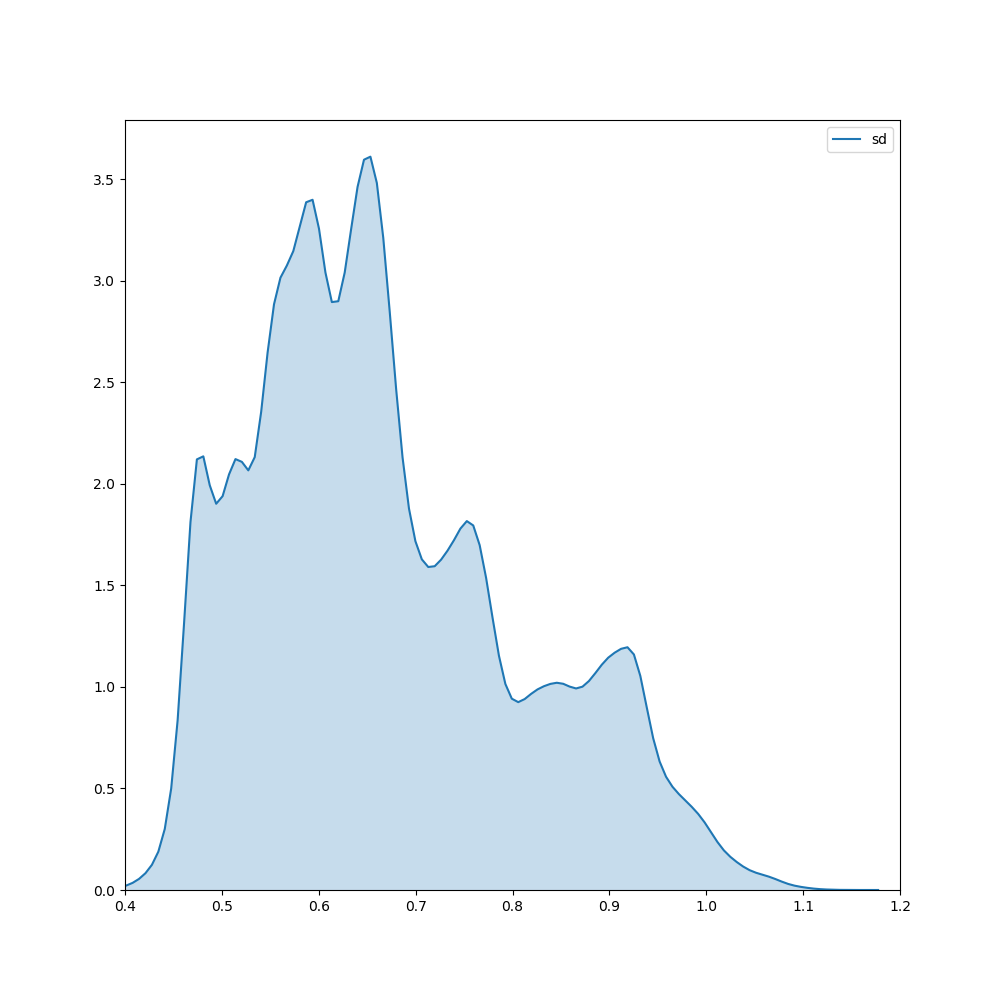
\includegraphics{../30_results/all_districts_concat_sd.png}
\caption{Spatial diversity of all districts \label{sd_all_districts}}
\end{figure}

A tempting conclusion to draw from the data is that these districts are
equally distributed over the different states. In reality, though, the
districts of a state can only take on a small range of values no matter
how a districting plan is drawn. Figure \ref{sd_districts_binned}
demonstrates. The peaks imply a multimodal distribution where individual
districts are clustered around certain values and not others. This is
most starkly displayed in the states with only two districts. Despite
the fact that the redistricting algorithm is continuous, there is a
sharp bimodal distribution present in the states of Idaho and Maine, and
to a lesser degree Utah and New Hampshire.

This finding is somewhat surprising. It implies that even though the
MCMC algorithm explores the entire set of feasible districting plans,
any district in any feasible plan will take on a specific form. In other
words---no matter how one draws the plan, each district's spatial
diversity is largely pinned down by its state's political geography.
Some states have very spatially diverse districts, some states have very
homogeneous ones, and this is a function of their geography and not the
way the districts are drawn.

\begin{figure}
\centering
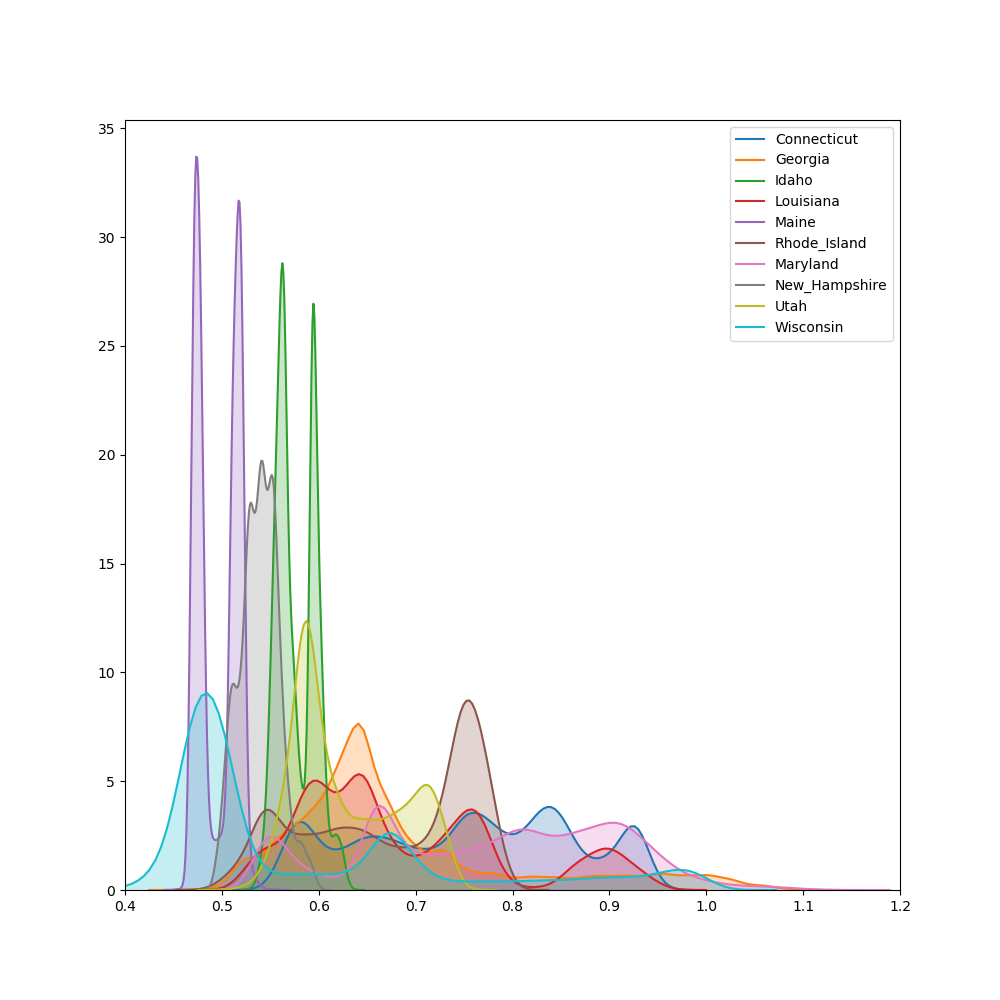
\includegraphics{../30_results/all_districts_sd.png}
\caption{Spatial diversity of districts binned by state
\label{sd_districts_binned}}
\end{figure}

Given that each district's spatial diversity is largely exogenous, we
should expect each state's overall spatial diversity not to vary much as
well. Indeed, we see in Figure \ref{sd_plans} that each state occupies a
narrow band in the range of possible spatial diversity scores. While the
range of spatial diversity scores ranges from 0.50 to 0.80, the range of
a state's spatial diversity score is only 0.05. While this range is
small, it is not insignificant. Figure \ref{sd_responsiveness} shows
that an increase in a state's spatial diversity by 0.05 is correlated
with a decrease in electoral responsiveness by 0.3, about 10\% of the
variance.

\begin{figure}
\centering
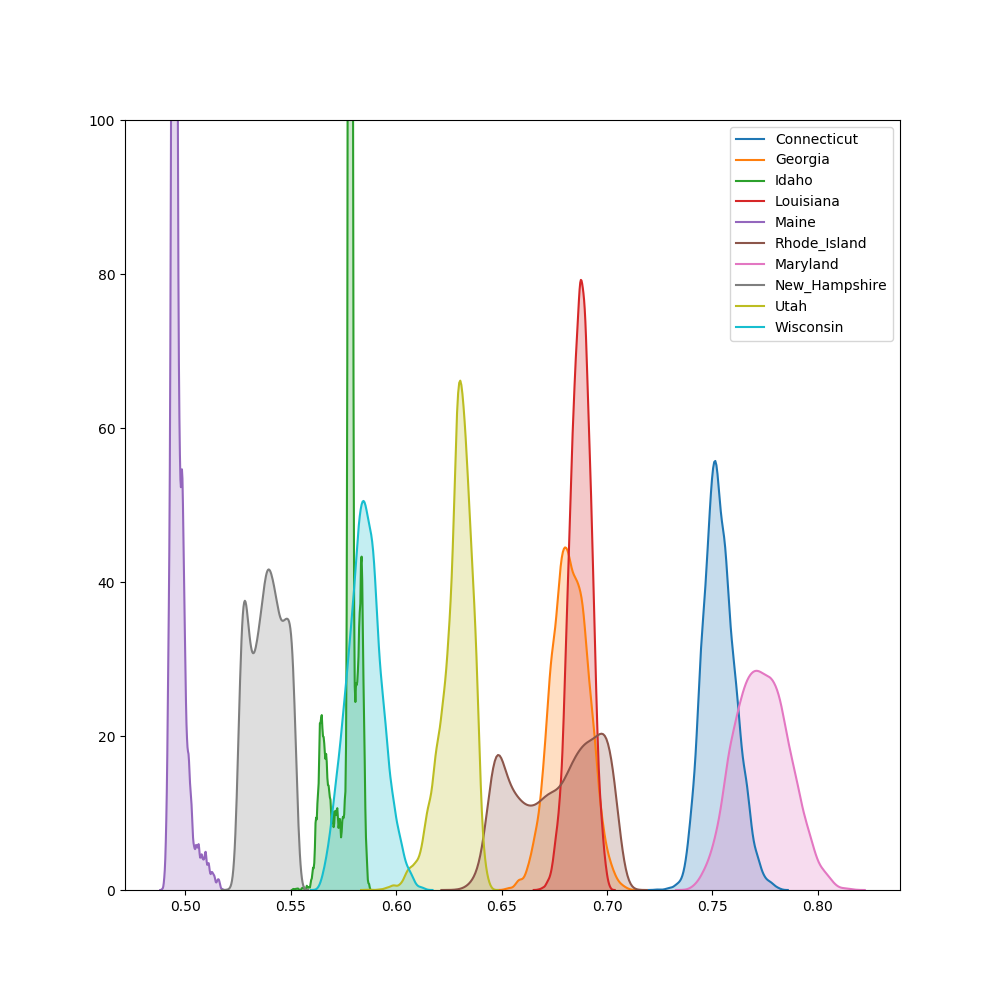
\includegraphics{../30_results/all_plans_sd.png}
\caption{Overall spatial diversity of districting plans by state
\label{sd_plans}}
\end{figure}

\hypertarget{districts-that-are-small-and-urban-are-usually-more-spatially-diverse}{%
\paragraph{Districts that are small and urban are usually more spatially
diverse}\label{districts-that-are-small-and-urban-are-usually-more-spatially-diverse}}

One finding consistent across all states is that the smaller (by area)
the district, the higher the spatial diversity.

\begin{figure}
\centering
\includegraphics{../30_results/22_pairwise_plot.png}
\caption{Pairwise plot of Maryland's districts: urban districts have
highest SD \label{pairwise_plot}}
\end{figure}

Maryland provides the clearest example, although the same pattern
repeats in all other states. Figure \ref{pairwise_plot} is a
correlation- and KDE plot of different metrics, binned by the area of
each district. The most important figure is the KDE plot in the top
left-hand corner. We can see that large districts (in blue) occupy the
low end of the spatial diversity range. Medium-sized districts (orange)
have a bimodal distribution, but it is the smallest districts (in green)
that have the highest spatial diversity.

This finding is quite intuitive. Cities tend to be the most
heterogeneous parts of a state, with people of different races, ages,
and socioeconomic classes. This finding suggests that more urban states
will simply have larger spatial diversity scores---another factor
pinning down the spatial diversity of a state's districting plans.

\hypertarget{conclusions-of-initial-data-exploration}{%
\paragraph{Conclusions of initial data
exploration}\label{conclusions-of-initial-data-exploration}}

We have seen that the overall distribution of districts and plans lie
within a tight bound, largely determined by each state's political
geography. This suggests that while districting can exert an effect on
political outcomes, we should not expect optimising for compactness to
change spatial diversity very much.

\hypertarget{compactness-measures-largely-agree-with-one-another-but-human-compactness-less-so}{%
\subsubsection{Compactness measures largely agree with one another, but
human compactness less
so}\label{compactness-measures-largely-agree-with-one-another-but-human-compactness-less-so}}

The next key finding is that compactness measures largely agree with one
another, meaning that a proposed plan that scores highly on one
compactness metric will likely score highly on another. The correlations
are strongest between the three geometric compactness measures, and
lower (but still significantly positive) between the geometric and human
compactness measures.

This finding is somewhat intuitive---we would expect the different
geometric compactness measures to track each other very closely as they
are measuring very similar concepts. It is much less obvious, however,
that a purely geometric measure would agree with a metric that measures
driving durations between points. This result is encouraging because it
shows that these metrics are able to get at the same concept despite
having completely different theoretical backgrounds.

One way to find the relationship between compactness measures would be
to aggregate all the observations from each state into a pooled data
set, and calculate the pairwise correlations between all such
observations. However, looking at these aggregate results in this way
can be highly misleading, as a single outlier state can bias the
results. I therefore look at the correlations for each individual state
instead.

One way to visualise these correlations is through the use of a heatmap.
Figure \ref{connecticut_corr} plots the correlation coefficients between
each pair of metrics. Firstly, we can see the correlation coefficients
between spatial diversity (sd) and the compactness metrics. Here, it
seems like human compactness has a significant negative correlation with
spatial diversity, with the other compactness metrics having little
correlation. We can also see that the correlation between human
compactness and geometric compactness measures are somewhat lower
(\textasciitilde{}0.46) than the correlations between different
geometric measures.

\begin{figure}
\centering
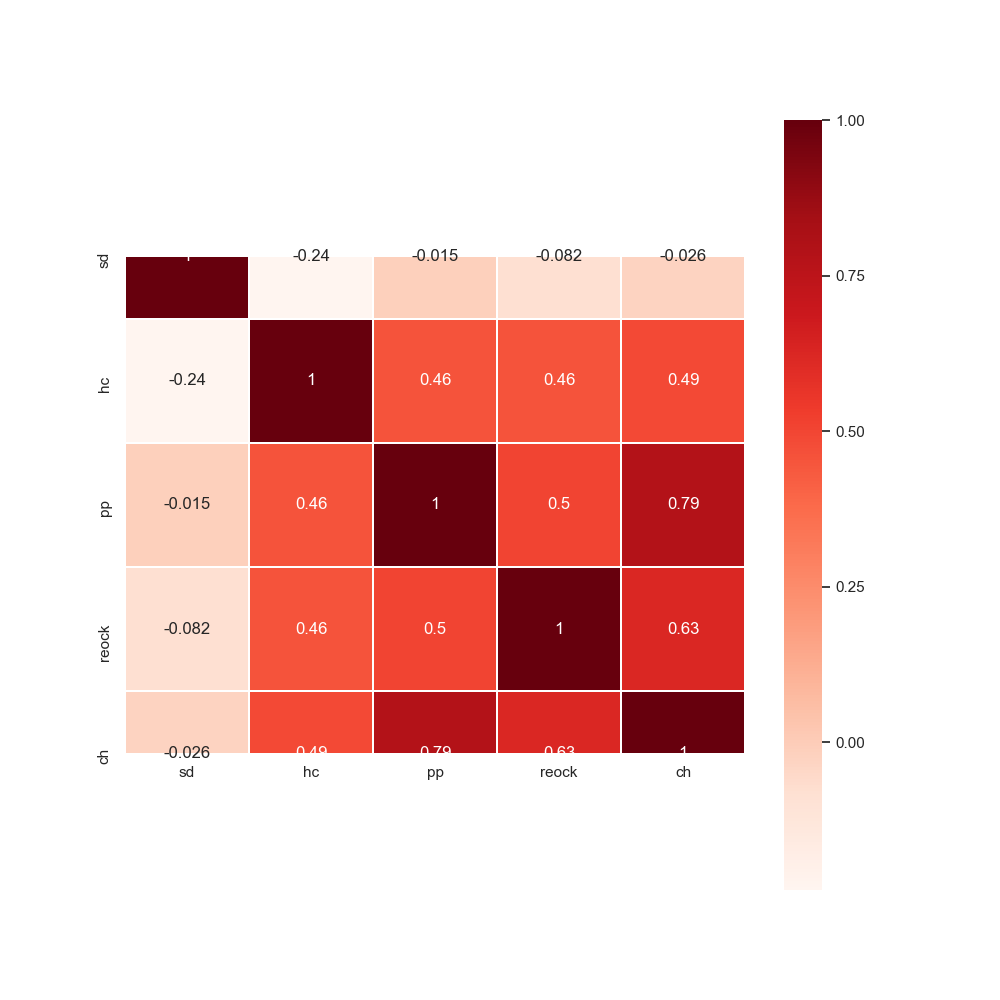
\includegraphics{../30_results/09_corr_matrix_grouped}
\caption{Correlation heatmap of Connecticut \label{connecticut_corr}}
\end{figure}

The correlation heatmap of Utah shows a case where human compactness and
the other geometric measures disagree. Here, the correlation between
geometric compactness measures is very high (0.89---almost 1), but there
is in fact a negative correlation between human compactness and the
geometric measures.

\begin{figure}
\centering
\includegraphics{../30_results/44_corr_matrix_grouped}
\caption{Correlation heatmap of Utah}
\end{figure}

These results vindicate my choice to use an ensemble of compactness
metrics rather than relying on a single measure. While the correlation
between metrics is high, it is not perfect, and indeed we observe cases
like Utah where the compactness measures disagree.

Another way to visualise the findings is through pairwise scatterplots.
Figure \ref{pairwise_plot_grouped} is a correlation plot between spatial
diversity and the various compactness metrics for the state of Georgia.
These plots have the advantage of being able to visualise the
scatterplots, which can surface non-linear relationships that a simple
correlation coefficient cannot. In all of the states, however, the
relationship between compactness metrics is always linear.

\begin{figure}
\centering
\includegraphics{../30_results/13_pairwise_plot_grouped.png}
\caption{Correlation plot of Georgia\label{pairwise_plot_grouped}}
\end{figure}

I have included correlation matrices and pairwise scatterplots for all
ten states in the Supplementary Information. The overall correlation is
positive for most states and most metrics, with human compactness being
less correlated with the other metrics.

\hypertarget{only-human-compactness-has-a-significant-negative-effect-on-spatial-diversity.}{%
\subsubsection{Only human compactness has a significant negative effect
on spatial
diversity.}\label{only-human-compactness-has-a-significant-negative-effect-on-spatial-diversity.}}

In this section, I run multivariate OLS regressions with country
dummies, as well as difference-in-means tests, and find no significant
effects of geometric compactness on spatial diversity. I find that human
compactness has a significant negative effect on spatial diversity:
increasing human compactness from 0 to 1 decreases spatial diversity by
0.04 points.

\hypertarget{multivariate-regression-with-country-dummies}{%
\paragraph{Multivariate regression with country
dummies}\label{multivariate-regression-with-country-dummies}}

We cannot simply run a regression aggregating every single district as
each state has a unique distribution of spatial diversity and
compactness. Consider the following. Within each state, increasing
compactness decreases spatial diversity. But on the aggregate, states
with high spatial diversity also have low compactness. In this case,
regressing spatial diversity on the aggregate level would give an
inflated estimate of the actual effect, falling afoul of the
\emph{ecological fallacy}. I illustrate this in figures \ref{indiv_reg}
and \ref{grouped_reg}. In Figure \ref{indiv_reg}, I plot a graph of
human compactness on the x-axis and spatial diversity on the y-axis. The
overall trend seems to be slightly negative: in most of the groups,
there is a slight negative correlation between human compactness and
spatial diversity. However, we would obtain erroneous results if we
aggregated the different states and ran a singular regression. This is
depicted in Figure \ref{grouped_reg}: due to the \emph{between-group}
correlation of compactness and spatial diversity, the estimate of the
effect is biased. We must therefore control for state when running the
regression. Thus, I run a multivariate regression with the functional
form \[SpatialDiversity = \beta_0 + \beta_1
Compactness + \beta_2 State\] where \(State\) is a dummy variable,
taking care to avoid the dummy variable trap.

Table \ref{table:ols_sd_hc} shows the results for human compactness. I
run the same regression for each compactness metric and obtain the
following:

\begin{verbatim}
HC: -0.0404, t-value -40.632
PP: +0.0251, t-value 29.841
Reock: +0.0209, t-value 27.645
CHull: -0.0016, t-value -1.801
\end{verbatim}

I find that only human compactness has a statistically significant
negative coefficient on spatial diversity, while Polsby-Popper and Reock
have a significant positive effect on spatial diversity. This initial
result suggests two things: firstly, and rather disappointingly, that
optimising over the two most popular compactness measures may have
adverse effects on electoral competitiveness and responsiveness. More
encouragingly, though, these effects can be mitigated by the judicious
choice of compactness measure. The results show that optimising over
Convex Hull does not come at the cost of diversity, and that increasing
human compactness actually decreases spatial diversity.

\begin{figure}
\centering
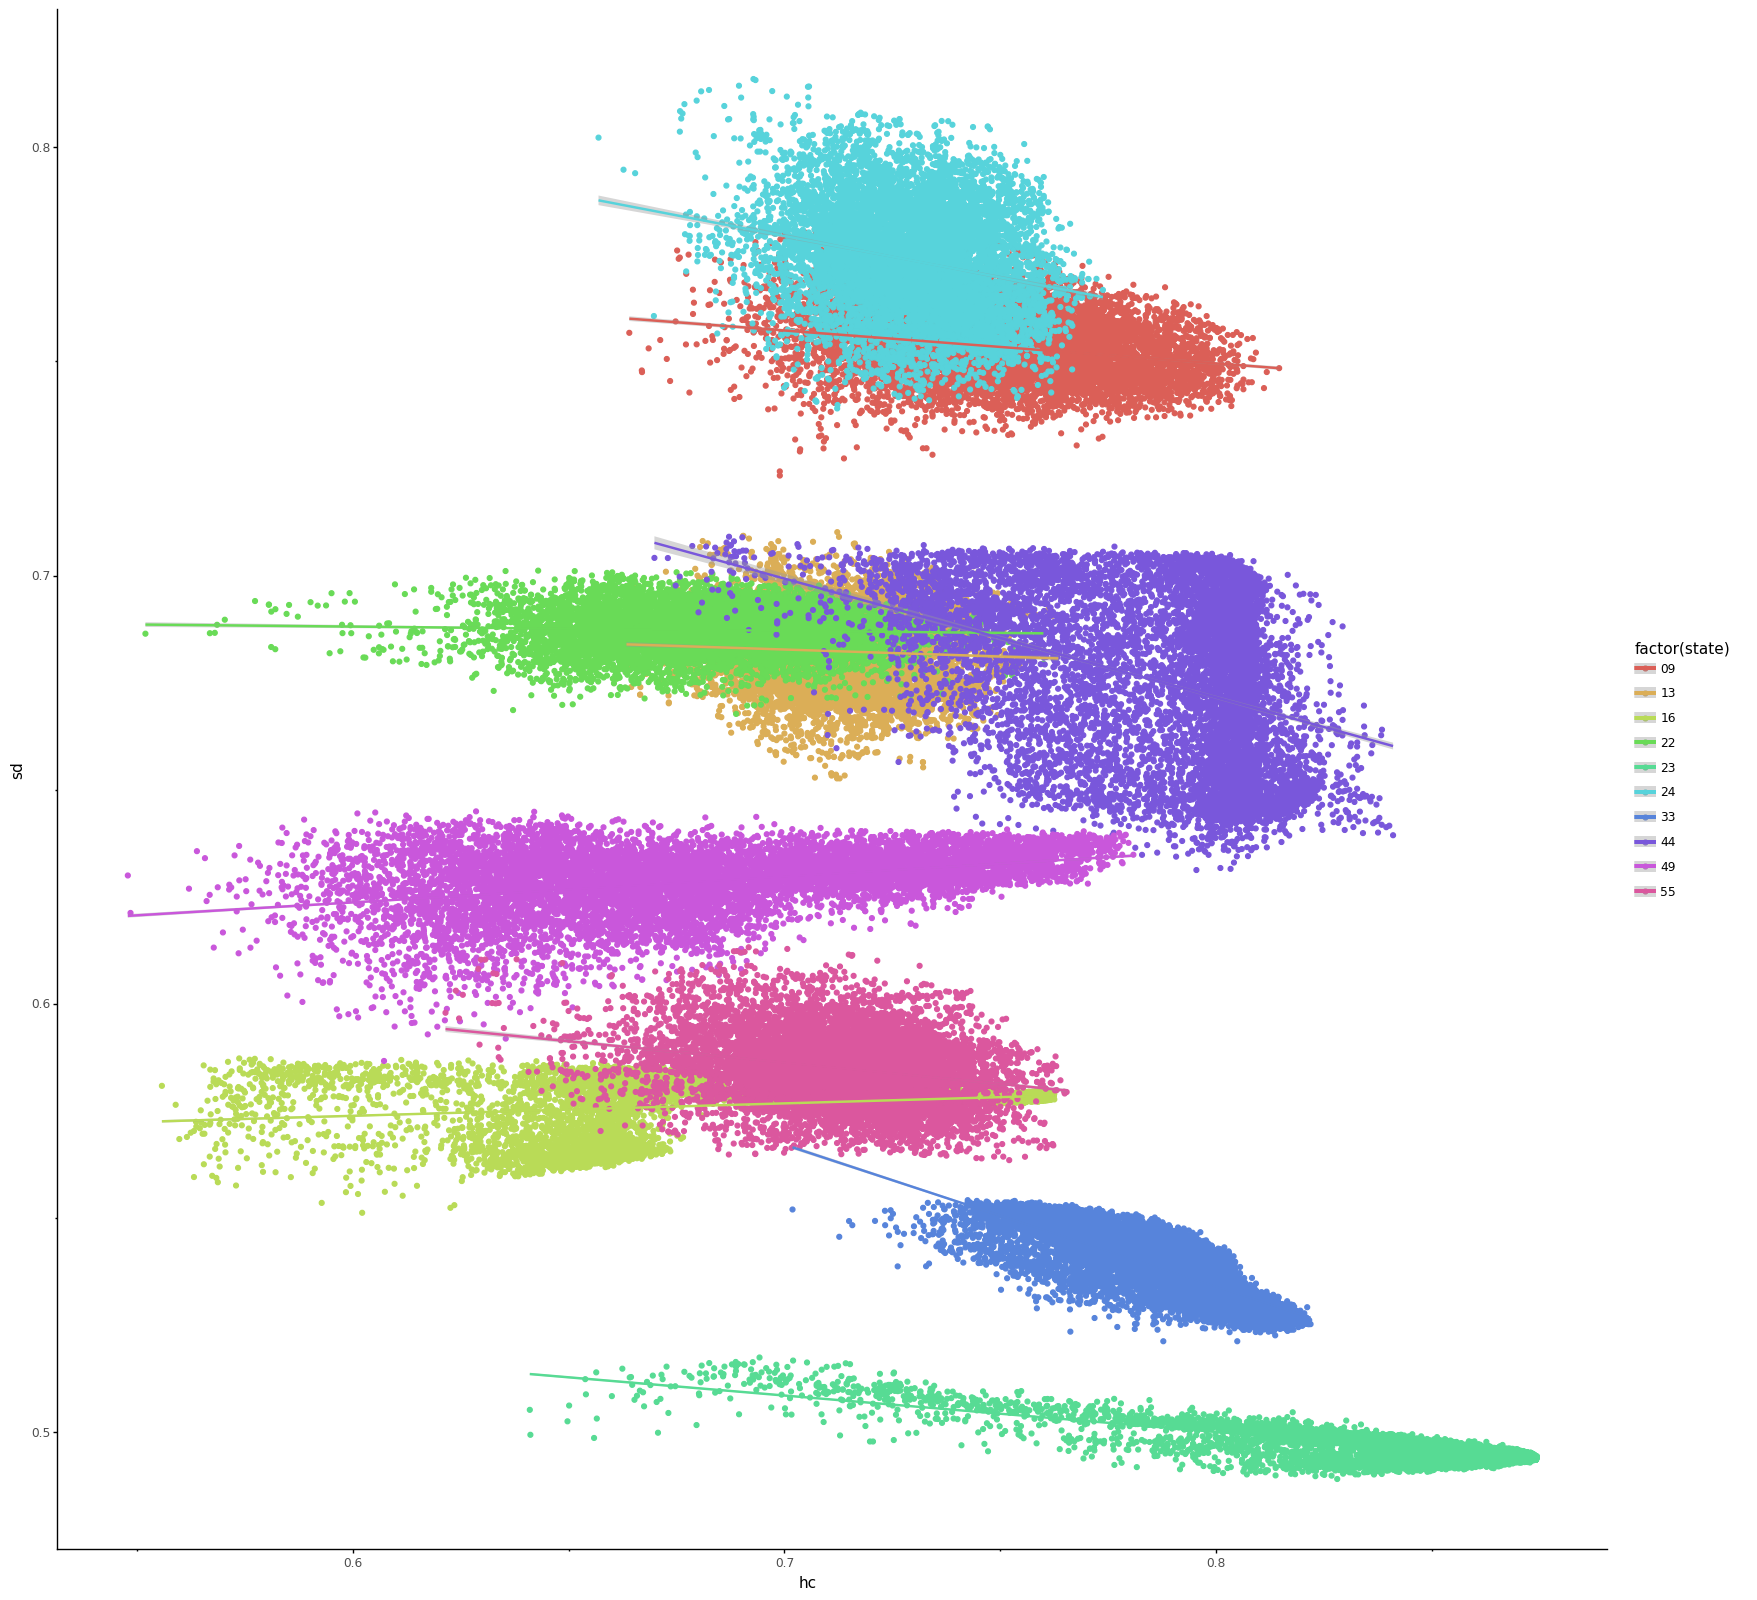
\includegraphics{../30_results/individual_regressions.png}
\caption{The individual-level regressions show a weak downward trend
between human compactness and spatial diversity\label{indiv_reg}}
\end{figure}

\begin{figure}
\centering
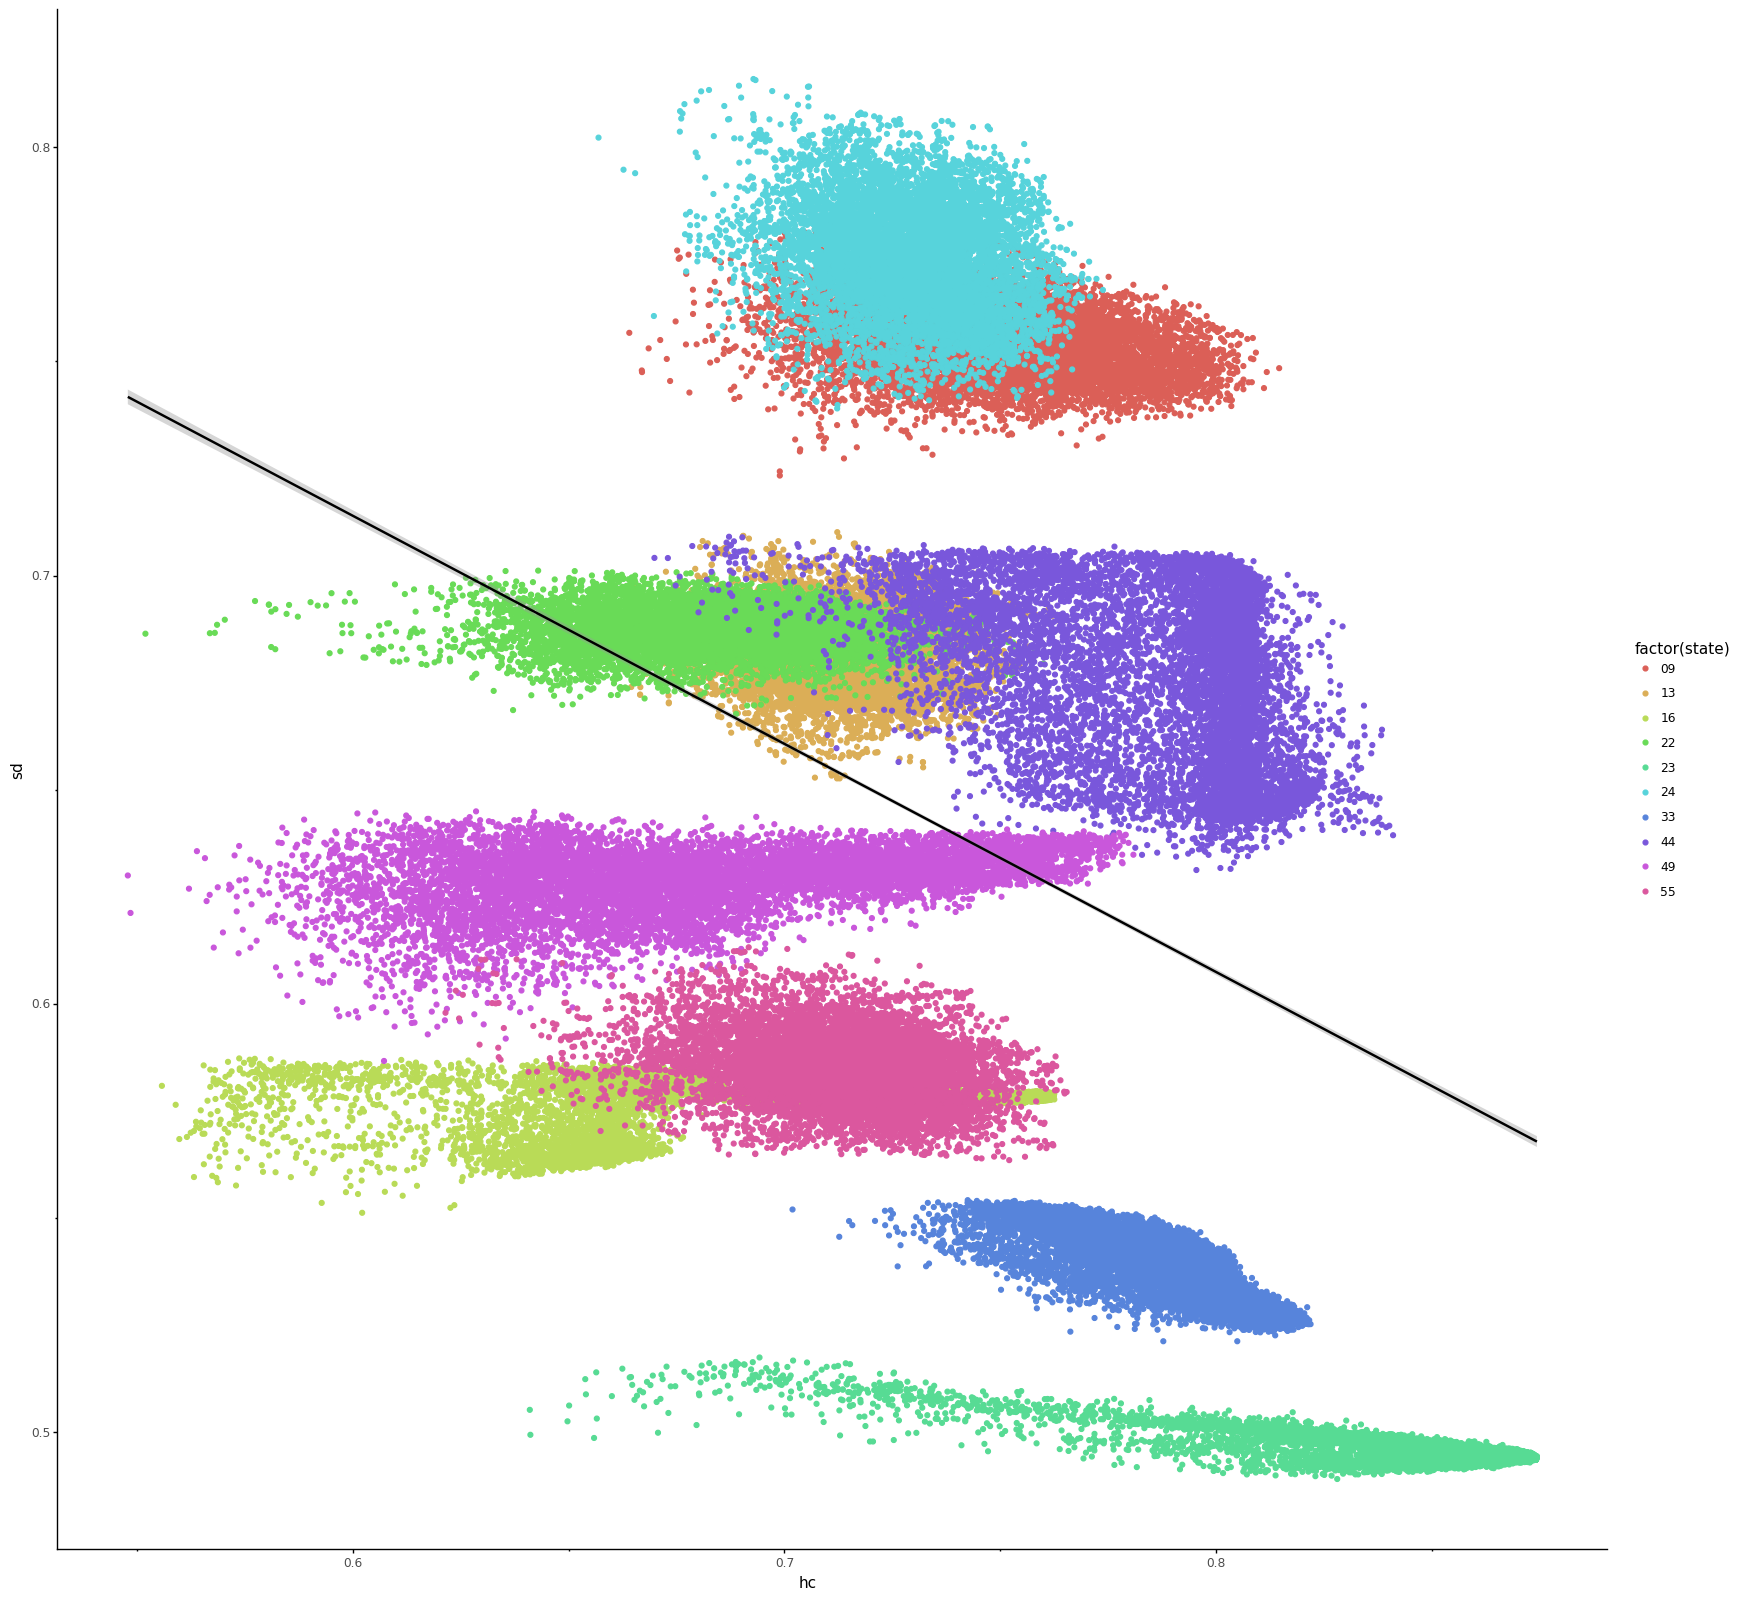
\includegraphics{../30_results/grouped_regressions.png}
\caption{Aggregating the individual states gives an inflated estimate of
the effect of compactness and commits the ecological fallacy
\label{grouped_reg}}
\end{figure}

\begin{table}[h!] 
\begin{center}
\caption{OLS Regression of Spatial Diversity on Human Compactness with
Country Dummies}
\label{table:ols_sd_hc}
\begin{tabular}{lclc}
\toprule
\textbf{Dep. Variable:}    &        sd        & \textbf{  R-squared:         } &     0.988   \\
\textbf{Model:}            &       OLS        & \textbf{  Adj. R-squared:    } &     0.988   \\
\textbf{Method:}           &  Least Squares   & \textbf{  F-statistic:       } & 8.188e+05   \\
\textbf{Date:}             & Wed, 11 Mar 2020 & \textbf{  Prob (F-statistic):} &     0.00    \\
\textbf{Time:}             &     20:23:45     & \textbf{  Log-Likelihood:    } & 3.2365e+05  \\
\textbf{No. Observations:} &      100000      & \textbf{  AIC:               } & -6.473e+05  \\
\textbf{Df Residuals:}     &       99989      & \textbf{  BIC:               } & -6.472e+05  \\
\textbf{Df Model:}         &          10      & \textbf{                     } &             \\
\bottomrule
\end{tabular}
\begin{tabular}{lcccccc}
                      & \textbf{coef} & \textbf{std err} & \textbf{t} & \textbf{P$> |$t$|$} & \textbf{[0.025} & \textbf{0.975]}  \\
\midrule
\textbf{C(state)[09]} &       0.7837  &        0.001     &  1042.069  &         0.000        &        0.782    &        0.785     \\
\textbf{C(state)[13]} &       0.7111  &        0.001     &   993.725  &         0.000        &        0.710    &        0.713     \\
\textbf{C(state)[16]} &       0.6054  &        0.001     &   856.490  &         0.000        &        0.604    &        0.607     \\
\textbf{C(state)[22]} &       0.7149  &        0.001     &  1039.373  &         0.000        &        0.714    &        0.716     \\
\textbf{C(state)[23]} &       0.5303  &        0.001     &   626.929  &         0.000        &        0.529    &        0.532     \\
\textbf{C(state)[24]} &       0.8030  &        0.001     &  1097.735  &         0.000        &        0.802    &        0.804     \\
\textbf{C(state)[33]} &       0.5705  &        0.001     &   725.232  &         0.000        &        0.569    &        0.572     \\
\textbf{C(state)[44]} &       0.7073  &        0.001     &   899.177  &         0.000        &        0.706    &        0.709     \\
\textbf{C(state)[49]} &       0.6561  &        0.001     &   959.927  &         0.000        &        0.655    &        0.657     \\
\textbf{C(state)[55]} &       0.6138  &        0.001     &   858.803  &         0.000        &        0.612    &        0.615     \\
\textbf{hc}           &      -0.0404  &        0.001     &   -40.632  &         0.000        &       -0.042    &       -0.038     \\
\bottomrule
\end{tabular}
\begin{tabular}{lclc}
\textbf{Omnibus:}       & 3979.140 & \textbf{  Durbin-Watson:     } &    1.171  \\
\textbf{Prob(Omnibus):} &   0.000  & \textbf{  Jarque-Bera (JB):  } & 9332.569  \\
\textbf{Skew:}          &  -0.236  & \textbf{  Prob(JB):          } &     0.00  \\
\textbf{Kurtosis:}      &   4.420  & \textbf{  Cond. No.          } &     67.9  \\
\bottomrule
\end{tabular}
\end{center}
\end{table}

\hypertarget{only-under-human-compactness-do-top-plans-have-lower-spatial-diversity-than-average}{%
\paragraph{Only under human compactness do top plans have lower spatial
diversity than
average}\label{only-under-human-compactness-do-top-plans-have-lower-spatial-diversity-than-average}}

While the results of the overall regression are discouraging, it may not
be the last word. The neutral ensemble approach means that the generated
plans run the whole gamut of compactness scores, including both highly
compact plans and highly noncompact ones in the sample of 100,000. In
reality, though, legislators will try to optimise for compactness to
some degree. A plan proposed in real life---while not being optimally
compact---would be reasonably so. Rather than regressing over the entire
sample, then, we should specifically check the spatial diversity of
plans which exceed the threshold of ``reasonable compactness''.

But what is the threshold of ``reasonable compactness''? The choice of
the threshold cannot be determined \emph{a priori}. One would have to
know the distribution of compactness in a sample of plans generated in
real life. Of course, as real-life expert districtors do not produce a
distribution of plans, this is also a tall order. I therefore run the
same OLS regression for different thresholds of ``reasonable
compactness'', ranging from the top 90\% (excluding the bottom 10\%) of
plans to the top 10\% of plans.\footnote{The results are similar when we
  take the top 5\% or 2\% of plans, but the small sample sizes of those
  thresholds mean that it is difficult to get statistical significance.}
The results are as follows:

\begin{verbatim}
10th percentile:
                   coef    std err          t      P>|t|
hc              -0.0256      0.001    -19.660      0.000
pp               0.0339      0.001     34.757      0.000
reock            0.0287      0.001     34.723      0.000
ch              -0.0001      0.001     -0.143      0.886

25th percentile:
                   coef    std err          t      P>|t|
hc              -0.0274      0.002    -16.018      0.000
pp               0.0357      0.001     30.861      0.000
reock            0.0307      0.001     33.635      0.000
ch              -0.0024      0.001     -2.153      0.031

50th percentile:
                   coef    std err          t      P>|t|
hc              -0.0514      0.003    -15.722      0.000
pp               0.0154      0.001     10.269      0.000
reock            0.0267      0.001     24.400      0.000
ch              -0.0119      0.001     -8.627      0.000

75th percentile:
                   coef    std err          t      P>|t|
hc              -0.1154      0.007    -17.023      0.000
pp              -0.0338      0.002    -14.814      0.000
reock            0.0185      0.002     12.136      0.000
ch              -0.0589      0.002    -30.961      0.000

90th percentile:
                   coef    std err          t      P>|t|
hc              -0.0396      0.013     -3.098      0.002
pp               0.0412      0.005      7.756      0.000
reock            0.0074      0.003      2.285      0.022
ch              -0.0274      0.004     -6.862      0.000
\end{verbatim}

The results vary somewhat depending on our choice of threshold, but are
on the whole remarkably consistent. The Reock measure performs poorly in
all thresholds. The Polsby-Popper metric is not much better either. Only
when the threshold is set to the top 25\% of plans does the coefficient
go below 0, and the effect reverses when we look at the top 10\% of
plans. I am inclined to believe that is an outlier. The Convex Hull
metric is the best of the dispersion-based metrics. It consistently has
a negative coefficient, although the negative coefficients are very
small---particularly when the threshold is low. Finally, the human
compactness metric performs well on all subsamples. The coefficient on
human compactness is larger than all the other metrics on all the
thresholds---a strong indication that it is the metric that best
minimises spatial diversity.

\hypertarget{the-average-spatial-diversity-of-top-plans-under-human-compactness-is-significantly-lower-than-the-average-spatial-diversity-of-top-plans-under-other-compactness-metrics}{%
\paragraph{The average spatial diversity of top plans under human
compactness is significantly lower than the average spatial diversity of
top plans under other compactness
metrics}\label{the-average-spatial-diversity-of-top-plans-under-human-compactness-is-significantly-lower-than-the-average-spatial-diversity-of-top-plans-under-other-compactness-metrics}}

The OLS regressions we run give the relationship between compactness and
spatial diversity. But perhaps one is not concerned about the marginal
effect of compactness on diversity. One might ask a more basic question:
if we mandate that plans are ``reasonably compact''---whatever that
means---and force legislators to propose only plans that cross a
threshold of reasonable compactness, will that adversely affect spatial
diversity?

If there is indeed a fundamental trade-off between compactness and
spatial diversity, then we should observe the average spatial diversity
of highly compact plans to be higher than the spatial diversity across
all plans. I therefore compare the mean spatial diversity of top 500
plans under each compactness metric to the mean spatial diversity of all
plans. As a robustness check, I look at different proportions (top
10\%/5\%/2\%) and obtain almost-identical results. The results are as
follows:

\begin{verbatim}
Mean SD of plans with highest Human Compactness scores: 0.635558
Mean SD of plans with highest Polsby-Popper scores: 0.640954
Mean SD of plans with highest Reock scores: 0.639897
Mean SD of plans with highest Convex Hull scores: 0.639985
Mean SD of all plans: 0.639758
\end{verbatim}

Encouragingly, there seems to be no trade-off between compactness and
spatial diversity: the mean spatial diversity in top compactness plans
is not higher than the overall mean spatial diversity. But only human
compactness has a mean spatial diversity \emph{significantly lower} than
the mean spatial diversity of all plans. In order to check the
significance of this result, I run a differences-in-means test using
Welch's t-test. I use Welch's t-test as Student's t-test relies on a
homogeneity in variances assumption. When the assumption of equal
variances is not met, Student's t-test yields unreliable results, while
Welch's t-test controls Type 1 error rates as expected
\citep{delacre2017}. In this case, since the top plans come from
different distributions, it is unlikely that the variances are
homogeneous. The results are as follows:

\begin{verbatim}
Welch's t-tests for the top 5% of plans

HC vs All: statistic=[-3.36526759]), pvalue=[0.00076992]
Reock vs All: statistic=[0.97597048]), pvalue=[0.32912173]
PP vs All: statistic=[0.11228718]), pvalue=[0.91059979]
CHull vs All: statistic=[0.18211076]), pvalue=[0.85550249]
\end{verbatim}

Only human compactness had a statistically significant difference in
mean spatial diversity. For completeness, I also ran pairwise
differences-in-means tests between all four metrics, for a total of 6
tests. The results are as follows:

\begin{verbatim}
Welch's t-tests for the top 5% of plans (significant results only)

HC vs PP: statistic=[-3.16361084]), pvalue=[0.00156292]
HC vs Reock: statistic=([-2.53127357]), pvalue=[0.01138011]
HC vs CHull: statistic=[-2.57101923]), pvalue=array([0.0101543]))
\end{verbatim}

As expected, there were no significant differences in means between any
of the geometric compactness metrics, but there was a significant
difference in the means between human compactness and the other
compactness metrics. Similar results obtain when I rerun the tests for
the top 10\% and top 2\% of plans under each compactness metric. The
results show that the top plans under human compactness have
significantly lower spatial diversity than the top plans under other
compactness metrics.

\begin{center}\rule{0.5\linewidth}{\linethickness}\end{center}

While this analysis is suggestive, there are two rejoinders to this.
Firstly, one could argue that the difference in means is quite small:
only 1.5\% of the total variance in spatial diversity. Secondly, one
might think that looking only at the aggregated results could be
misleading. A difference in means in the aggregate could be due to one
or a few outlier states driving the results.

To address these two criticisms, I run Welch's t-tests for each metric
for all ten states (giving a total of 40 t-tests). The full list of
t-tests is available in Appendix B. Once again, human compactness
performs the best. The top plans under the Reock metric have
statistically significant negative differences in spatial diversity
means in 3 out of 10 states. Polsby-Popper and Convex Hull do a little
better with 4 out of 10 states. Human Compactness has a whopping seven
states. If we look at \emph{meaningful} differences---not just
statistically significant ones (instances where the mean is lower by
more than 5\% of the total variance)---then human compactness
outperforms by a wide margin. Human compactness has a statistically
significant and meaningfully lower spatial diversity in six of the
states. Reock does in two states, and Convex Hull and Polsby-Popper only
in one. Finally, in two cases (both under the human compactness metric),
the difference is so meaningful that it makes up 25\% and 35\% of the
total variance. Concretely, the spatial diversity of all 10,000 New
Hampshire plans lie within a range of 0.03. The top 1,000 plans under
human compactness have a spatial diversity that is 0.01 lower than the
mean --- a very meaningful effect that spans one-third of the total
range. Far from being a small effect, it seems that the choice of
compactness metric to optimise over can have very meaningful impacts.

What do the difference in means actually imply in terms of proposed
plans? Table \ref{table:top_plans_sd_percentile} shows what percentile
the top 10 percent of plans under each metric would occupy in the
distribution of 10,000 plans (lower is better). If there is no
relationship between a compactness metric and spatial diversity, then we
should expect the mean percentile to lie around 50 percent. If, however,
the top plans under a metric are significantly less spatially diverse,
then we should see a low percentile for many of the states. In the
table, I have \textbf{bolded} the best-performing metric in each row,
subject to it being less than the median (\textless{}50th percentile).
As before, I run robustness checks and get qualitatively similar results
for various threshold cut-offs.

\begin{table}[h!]
\begin{center}
\caption{What percentile the top 10 percent of plans under each metric occupy (lower is better)}
\label{table:top_plans_sd_percentile}
\begin{tabular}{lrrrr}
\toprule
{} &     hc &     pp &  reock &     ch \\
\midrule
0 Connecticut &  \textbf{34.31} &  54.02 &  55.61 &  48.25 \\
1 Georgia &  48.29 &  \textbf{44.24} &  48.34 &  47.62 \\
2 Idaho &  59.92 &  48.62 &  \textbf{20.90} &  26.88 \\
3 Louisiana &  \textbf{39.03} &  39.12 &  42.45 &  41.24 \\
4 Maine &  26.22 &  92.48 &  78.12 &  \textbf{23.56} \\
5 Rhode Island &  \textbf{23.32} &  56.46 &  53.71 &  52.70 \\
6 Maryland &  36.99 &  \textbf{33.00} &  33.00 &  48.68 \\
7 New Hampshire &   \textbf{8.25} &  58.08 &  40.30 &  65.73 \\
8 Utah &  77.05 &  61.72 &  58.57 &  59.92 \\
9 Wisconsin &  \textbf{34.09} &  42.14 &  47.26 &  43.07 \\
\bottomrule
Mean percentile & \textbf{38.75} &  52.99  &  47.83 &  45.77 \\
\bottomrule
\end{tabular}
\end{center}
\end{table}

The table shows that the human compactness metric consistently
outperforms the other metrics in many of the states, forestalling the
criticism that the results may be driven by one or two outliers. While
human compactness does particularly well in New Hampshire and Rhode
Island, it still performs best overall even if we remove those two
states from consideration.

\hypertarget{discussion-and-directions-for-future-work}{%
\subsection{Discussion and directions for future
work}\label{discussion-and-directions-for-future-work}}

\hypertarget{is-there-a-trade-off-between-compactness-and-spatial-diversity}{%
\subsubsection{Is there a trade-off between compactness and spatial
diversity?}\label{is-there-a-trade-off-between-compactness-and-spatial-diversity}}

Is there a fundamental trade-off between compactness and district
homogeneity (spatial diversity)? The answer seems to be: it depends on
how you measure compactness. For geometric compactness measures, the
results are equivocal: OLS regressions indicate that there is some
trade-off between compactness and homogeneity, while difference-in-means
tests indicate no such trade-off. Point-based distance metrics seem to
fare better. In fact the results show that rather than a trade-off,
there is a synergy between human compactness and district homogeneity.

It was certainly the right call to use an ensemble of compactness
metrics, due to the frequency at which even very similar compactness
measures disagree. The Maine entry in Table
\ref{table:top_plans_sd_percentile} is a good example. The top
Polsby-Popper plans lie in the 92nd percentile of all plans---shockingly
high---but looking at the Reock and Convex Hull measures paint a much
less one-sided picture. In fact, it is surprising that the Reock and
Convex Hull percentiles differ so radically, seeing as the measures
differ only in the bounding shape (convex polygon versus a circle) of
the district.

If we had used only the Polsby-Popper metric in our analyses, we would
have (erroneously) concluded that Maine's political geography was
fundamentally incompatible with compactness. This casts doubt upon work
that uses only a singular compactness metric to score districting plans.
Without wishing to single out any work in particular (many other papers
do the same thing), \cite{s2020} uses only the Polsby-Popper measure to
analyse only two states. My data suggests that this analysis is
insufficient---severely curtailing the generalisability of the work.

\hypertarget{does-spatial-diversity-suggest-one-compactness-metric-over-another}{%
\subsubsection{Does spatial diversity suggest one compactness metric
over
another?}\label{does-spatial-diversity-suggest-one-compactness-metric-over-another}}

Does spatial diversity give us a good reason to choose one compactness
metric over another? Yes. The data show that human compactness better
tracks spatial diversity, which in turn correlates with democratic
outcomes like participation, responsiveness and competitiveness. This
finding consistently repeats itself throughout different analyses,
different thresholds, and different aggregation functions. The
implication is clear: if we believe Stephanopoulos's work on the
benefits of lower spatial diversity, then adopting human compactness
will give us better plans.

To be fair, there are many other considerations that go into choosing a
compactness metric, and I have alluded to several in the previous
sections. First is objectivity. Geometric compactness measures were
invented in the first place---almost six decades ago---to measure and
prosecute gerrymandering objectively: ``{[}compactness{]} remains
subjective in that no method of measurement has gained general
acceptance'' \citep[p.~74]{reock1961}.

But second---and possibly far more important---is explainability.
Compactness metrics feature prominently in spheres outside academic
political science, from general political discourse to amicus briefs for
the Supreme Court. The seminal work by Reock almost sixty years ago says
``the best use for the method of measuring compactness outlined here is
\emph{as a tool for the courts and as a weapon for public opinion}''. It
is thus incredibly important that a compactness metric be intuitive and
explainable to the laymen. This almost entirely rules out overly
mathematical measures like \cite{dc2016} that use graph theory and
minimise cut edges, or uninterpretable measures like \cite{kingwp} that
build a ``black box'' machine learning model.

While geometric compactness metrics are simple enough to explain, they
lack a normative appeal. It is almost too easy to criticise geometric
compactness metrics on the basis of irrelevance. If we ask: \emph{why}
should districts follow some regular shape? the answer is not
immediately forthcoming, and in fact many have pointed out correctly
that there is little reason to do so \emph{eo ipso}.

Human compactness seems to meet both these criteria. It encapsulates the
notion of ``communities of interest'', while sidestepping the problem of
having to define, delineate and make subjective judgement calls on these
communities. And while it's not obvious that districts should conform to
some regular polygon, the idea of putting people who live together in
the same voting district has a strong normative force with great
intuitive appeal. Finally, the lower (but still substantially positive)
correlation between human compactness and the other compactness measures
suggests that human compactness qualitatively differs from geometric
compactness.

\hypertarget{directions-for-future-work}{%
\subsubsection{Directions for future
work}\label{directions-for-future-work}}

Future work should look at expanding the scope of the analysis in three
ways: the number of states, the number of compactness measures, and the
number of outcomes of interest.

My work analyses 10 out of the 50 states. Restricting analysis to a
subset of states is common in other redistricting work, due to the
onerous computational burdens of the procedure. \cite{ddj2019comp}
measure the effect of competitiveness on partisanship for five states,
and \cite{s2020} looks at the trade-off between compactness and partisan
symmetry for only two states. We know, however, that this has
implications on external validity. While my analysis covers more states
than much of the literature, further work should nonetheless extend the
analysis to cover more states---especially large states like Texas,
Florida and California.

Future work should also analyse more compactness measures. Of particular
interest would be other point-wise distance metrics like bizarreness,
and \citeauthor{kingwp}'s (\citeyear{kingwp}) metric that attempts to
imitate human perception.

Finally, future work should analyse a variety of other outcomes of
interest apart from spatial diversity. As the primary draw of
point-based distance measures is that it should keep communities of
people togetherin the same district, I would particularly like to see
future work whether human compactness does a better job of keeping
communities of interest together. We should also examine the effect of
compactness on a wider range of normative outcomes---not just procedural
ones. Districting affects many other things: political knowledge,
turnout, and federal spending \citep{snyder2010}, but work so far has
been placed almost entirely on electoral competitiveness.

\hypertarget{conclusion}{%
\subsubsection{Conclusion}\label{conclusion}}

{[}TODO{]}

\hypertarget{acknowledgements}{%
\subsection{Acknowledgements}\label{acknowledgements}}

\begin{itemize}
\tightlist
\item
  Big thanks to Bassel;
\item
  Big thanks to Daryl Deford, for explaining MCMC, Gerrychain, and
  generating the districting plans;
\item
  and Filip, for walking through with me all my ideas from May 2019
  until now;
\item
  and Stephanopoulos, for giving me his spatial diversity data;
\item
  Eubank and Rodden, for being kind enough to respond to my emails, and
  their VRP data,
\item
  Tak Huen, for giving me copies of \emph{Political Analysis}, from
  which the initial idea of this thesis came;
\item
  Zun Yuan, for letting me bounce optimisation ideas off him;
\item
  Sergi, for being the tutor that got me interested in Politics;
\item
  Am I allowed to thank Andy or name him as my supervisor? Ask Tak Huen
  about this
\end{itemize}

Images of Reock and PP metric taken from
\href{https://fisherzachary.github.io/public/r-output.html}{fisherzachary.github.io}

\hypertarget{appendix-a-explanation-of-human-compactness-metric}{%
\section{Appendix A: Explanation of human compactness
metric}\label{appendix-a-explanation-of-human-compactness-metric}}

Maybe not necessary, but talk about the precomputation steps and saving
the pointwise distances

\hypertarget{appendix-b-results-of-difference-in-means-tests-for-individual-states}{%
\section{Appendix B: Results of difference-in-means tests for individual
states}\label{appendix-b-results-of-difference-in-means-tests-for-individual-states}}

Here I compare the average spatial diversity of all 10,000 plans per
state to the average spatial diversity of the 500 most compact plans per
state.

I present the results for each state and each metric in the ensemble,
using Welch's t-test.

\begin{tabular}{lrlrrrrr}
\toprule
{} &  state & metric &  mean\_diff &  variance &  pct\_variance &      t-stat &        p-value \\
\midrule
0  &      0 &     hc &  -0.003460 &  0.058642 &     -5.900607 &  -17.425785 &   1.366961e-61 \\
1  &      0 &     pp &   0.000069 &  0.058642 &      0.118009 &    0.288166 &   7.732681e-01 \\
2  &      0 &  reock &   0.000381 &  0.058642 &      0.650317 &    1.624462 &   1.045297e-01 \\
3  &      0 &     ch &  -0.001042 &  0.058642 &     -1.776135 &   -5.014481 &   6.033771e-07 \\
4  &      1 &     hc &  -0.000513 &  0.057499 &     -0.892208 &   -1.868482 &   6.193359e-02 \\
5  &      1 &     pp &  -0.001423 &  0.057499 &     -2.475505 &   -4.986335 &   7.054193e-07 \\
6  &      1 &  reock &  -0.000498 &  0.057499 &     -0.865298 &   -1.692770 &   9.076060e-02 \\
7  &      1 &     ch &  -0.000678 &  0.057499 &     -1.178930 &   -2.231754 &   2.581874e-02 \\
8  &      2 &     hc &   0.001489 &  0.036047 &      4.131827 &   26.809567 &  2.038788e-153 \\
9  &      2 &     pp &   0.001104 &  0.036047 &      3.062205 &   10.321991 &   2.820313e-24 \\
10 &      2 &  reock &  -0.000188 &  0.036047 &     -0.520417 &   -0.859779 &   3.900941e-01 \\
11 &      2 &     ch &   0.000383 &  0.036047 &      1.063637 &    2.841225 &   4.560090e-03 \\
12 &      3 &     hc &  -0.001257 &  0.033457 &     -3.756204 &   -9.240446 &   9.523388e-20 \\
13 &      3 &     pp &  -0.001245 &  0.033457 &     -3.720159 &   -7.632057 &   4.670461e-14 \\
14 &      3 &  reock &  -0.000776 &  0.033457 &     -2.318159 &   -5.132091 &   3.320205e-07 \\
15 &      3 &     ch &  -0.000927 &  0.033457 &     -2.770633 &   -7.108140 &   1.896994e-12 \\
16 &      4 &     hc &  -0.001902 &  0.028376 &     -6.704063 &  -49.155427 &   0.000000e+00 \\
17 &      4 &     pp &   0.005131 &  0.028376 &     18.081320 &   38.153281 &  1.090249e-206 \\
18 &      4 &  reock &   0.001304 &  0.028376 &      4.596054 &   20.334160 &   7.714653e-84 \\
19 &      4 &     ch &  -0.002035 &  0.028376 &     -7.171113 &  -50.341694 &   0.000000e+00 \\
20 &      5 &     hc &  -0.019707 &  0.077819 &    -25.324736 &  -43.785027 &  7.817121e-271 \\
21 &      5 &     pp &   0.007385 &  0.077819 &      9.490310 &   14.029691 &   8.033314e-42 \\
22 &      5 &  reock &   0.005601 &  0.077819 &      7.197869 &   10.059549 &   5.666063e-23 \\
23 &      5 &     ch &   0.004848 &  0.077819 &      6.229592 &    8.615116 &   2.011837e-17 \\
24 &      6 &     hc &  -0.004913 &  0.076917 &     -6.386934 &  -12.541515 &   4.676097e-34 \\
25 &      6 &     pp &  -0.006333 &  0.076917 &     -8.233653 &  -16.445177 &   3.655560e-55 \\
26 &      6 &  reock &  -0.006334 &  0.076917 &     -8.235342 &  -17.317992 &   1.527167e-60 \\
27 &      6 &     ch &  -0.000795 &  0.076917 &     -1.033852 &   -1.809545 &   7.061978e-02 \\
28 &      7 &     hc &  -0.011556 &  0.032940 &    -35.083239 & -120.004988 &   0.000000e+00 \\
29 &      7 &     pp &   0.002150 &  0.032940 &      6.527335 &    9.218455 &   1.208411e-19 \\
30 &      7 &  reock &  -0.002165 &  0.032940 &     -6.573630 &  -11.615082 &   6.541658e-30 \\
31 &      7 &     ch &   0.004050 &  0.032940 &     12.294876 &   17.193270 &   1.023553e-59 \\
32 &      8 &     hc &   0.005538 &  0.058276 &      9.503582 &   42.778404 &  4.401068e-291 \\
33 &      8 &     pp &   0.002962 &  0.058276 &      5.082034 &   18.477814 &   2.578165e-69 \\
34 &      8 &  reock &   0.002492 &  0.058276 &      4.275665 &   14.864941 &   8.132217e-47 \\
35 &      8 &     ch &   0.002689 &  0.058276 &      4.613737 &   16.787183 &   1.984654e-58 \\
36 &      9 &     hc &  -0.003290 &  0.049699 &     -6.619743 &  -13.092609 &   8.687410e-37 \\
37 &      9 &     pp &  -0.001645 &  0.049699 &     -3.309711 &   -6.053633 &   1.889349e-09 \\
38 &      9 &  reock &  -0.000677 &  0.049699 &     -1.361577 &   -2.476624 &   1.340008e-02 \\
39 &      9 &     ch &  -0.001482 &  0.049699 &     -2.982079 &   -5.561983 &   3.278783e-08 \\
\bottomrule
\end{tabular}

\bibliography{references.bib}

\end{document}
